% `advanced_example.tex', an advanced example employing the AIAA class
% plus other third-party LaTeX packages.
%
% For a bare-bones usage, see `template.tex'.
%
% Typical processing for PostScript (PS) output:
%
%  latex advanced_example
%  bibtex advanced_example  (bibliography)
%  makeindex -s nomencl.ist -o advanced_example.gls advanced_example.glo
%                            (nomenclature)
%  latex advanced_example   (repeat as needed to resolve references)
%
%  xdvi advanced_example    (onscreen draft display)
%  dvips advanced_example   (postscript)
%  gv advanced_example.ps   (onscreen display)
%  lpr advanced_example.ps  (hardcopy)
%
% With the above, only Encapsulated PostScript (EPS) images can be used.
%
%
%  pdflatex advanced_example
%  bibtex advanced_example    (bibliography)
%  makeindex -s nomencl.ist -o advanced_example.gls advanced_example.glo
%                              (nomenclature)
%  pdflatex advanced_example  (repeat as needed to resolve references)
%
%  acroread advanced_example.pdf  (onscreen display)
%
% If you have EPS figures, you will need to use the epstopdf script
% to convert them to PDF because PDF is a limmited subset of EPS.
% pdflatex accepts a variety of other image formats such as JPG, TIFF,
% PNG, and so forth -- check the documentation for your version.
%
% If you do *not* specify suffixes when using the graphicx package's
% \includegraphics command, latex and pdflatex will automatically select
% the appropriate figure format from those available.  This allows you
% to produce PS and PDF output from the same LaTeX source file.
%
% To generate a large format (e.g., 11"x17") PostScript copy for editing
% purposes, use
%
%  dvips -x 1467 -O -0.65in,0.85in -t tabloid advanced_example
%
% For further details and support, read the Users Manual, aiaa.pdf.

\documentclass[]{aiaa-tc}% insert '[draft]' option to show overfull boxes

 \usepackage{varioref}%  smart page, figure, table, and equation referencing
 \usepackage{wrapfig}%   wrap figures/tables in text (i.e., Di Vinci style)
 \usepackage{threeparttable}% tables with footnotes
 \usepackage{dcolumn}%   decimal-aligned tabular math columns
  \newcolumntype{d}{D{.}{.}{-1}}
 \usepackage{nomencl}%   nomenclature generation via makeindex
  \makeglossary
 \usepackage{amssymb,amsmath}
 \usepackage{subfigure}% subcaptions for subfigures
 \usepackage{subfigmat}% matrices of similar subfigures, aka small mulitples
 \usepackage{fancyvrb}%  extended verbatim environments
 \fvset{fontsize=\footnotesize,xleftmargin=2em}
 \usepackage{lettrine}%  dropped capital letter at beginning of paragraph
%  \usepackage[dvips]{dropping}% alternative dropped capital package
 \usepackage[colorlinks]{hyperref}%  hyperlinks [must be loaded after dropping]
 \usepackage{float}
 \usepackage{longtable,booktabs,tabularx}
 \restylefloat{table}
 \usepackage{graphicx}
 \usepackage{caption}
 \usepackage{siunitx}
 \usepackage{multicol}
 \usepackage{indentfirst}
 \usepackage[labelfont=bf]{caption}

 \title{Solar-Electric and Gas Powered, Long-Endurance UAV Sizing via Geometric Programming}

 \author{
  Michael Burton \thanks{Master's Candidate, Aeronautical and Astronautical Engineering, 77 Mass Ave, Cambridge MA, 02139, AIAA Student.}
  \ and Warren Hoburg\thanks{Professor, Aeronautical and Astronautical Engineering, 77 Mass Ave, Cambridge MA, 02139, AIAA Member.}\\
  {\normalsize\itshape
   Massachusetts Institute of Technology, Cambridge, 02139, USA}\\
 }

 % Data used by 'handcarry' option
 \AIAApapernumber{YEAR-NUMBER}
 \AIAAconference{Conference Name, Date, and Location}
 \AIAAcopyright{\AIAAcopyrightD{YEAR}}

 % Define commands to assure consistent treatment throughout document
 \newcommand{\eqnref}[1]{(\ref{#1})}
 \newcommand{\class}[1]{\texttt{#1}}
 \newcommand{\package}[1]{\texttt{#1}}
 \newcommand{\file}[1]{\texttt{#1}}
 \newcommand{\BibTeX}{\textsc{Bib}\TeX}
 \usepackage{hyperref}
 \hypersetup{citecolor = blue}

\begin{document}

\maketitle

\begin{abstract}
    Using geometric programming, a comparison of solar-electric and gas powered, long-endurance aircraft is accomplished.
    Long-endurance aircraft present a complicated systems engineering problem because of the multifaceted interaction of various requirements, such as endurance, velocity and coverage footprint.
    Geometric programming, a form of convex optimization, can reliably solve problems with thousands of variables in seconds and is used as an optimization tool to evaluate the design trade offs between architectures and requirements.
    Using this approach, a gas powered and a solar-electric powered aircraft were considered.  
    The results show that long-endurance, gas powered aircraft are generally more robust to higher wind speeds than solar-powered aircraft.  
    However, gas powered aircraft are limited in their endurance by the amount of fuel that they can carry. 
    While solar-electric powered aircraft can theoretically fly for months, they are operationally limited by limited sunlight during the winter and wind speeds at higher latitudes.
    Using geometric programming, a detailed trade study between gas-powered and solar-powered aircraft is performed to discover which architecture is best suited to meet a given set of requirements, and what is the optimum size and endurance of that platform.
\end{abstract}

\section*{Nomenclature}

\begin{multicols}{2}
\small

\begin{tabbing}
  XXXXXXX \= \kill% this line sets tab stop
$A$ \> wing aspect ratio \\
$\bar{A}$ \> non-dimensional cross sectional area \\
$b$ \> wing span [ft] \\
$BSFC$ \> brake specific fuel consumption [lb/hr/hp] \\
$c$ \> wing chord [m] \\
$C_D$ \> drag coefficient \\
$C_{d_0}$ \> non-wing drag coefficient \\
$c_{d_{\text{h}}}$ \> horizontal tail profile drag coefficient \\
$c_{d_p}$ \> wing profile drag coefficient \\
$c_{d_{\text{v}}}$ \> vertical tail profile drag coefficient \\
$C_f$ \> skin friction coefficient \\
$C_L$ \> lift coefficient \\
$c_{l_{\alpha}}$ \> lift slope coefficient \\
$C_{L_{\text{max}}}$ \> maximum lift coefficient \\
$d$ \> tail boom diameter [m] \\
$D_{\text{boom}}$ \> tail boom drag [N] \\
$\Delta W$ \> wing section weight [N] \\
$\Delta y$ \> wing section length [m] \\
$DOY$ \> day of the year \\
$e$ \> Oswald efficiency factor \\
$E$ \> Young's Modulus [Pa] \\
$E_{\text{battery}}$ \> energy stored in battery [J] \\
$E_{\text{sun}}$ \> total solar energy available [Whr] \\
$(E/S)_{\text{sun}}$ \> available solar energy per unit area [Whr/m$^2$] \\
$f_{\text{solar}}$ \> planform area fraction covered in solar cells \\
$f_{\text{structural}}$ \> fractional structural weight\\
$g$ \> gravitational constant [m/s$^2$] \\
$h$ \> flight altitude [ft] \\
$h_{\text{batt}}$ \> battery energy density [Whr/kg] \\
$h_{\text{cap}}$ \> spar cap separation [m] \\
$I$ \> cap spar moment of inertia [m$^4$] \\
$I_0$ \> tail boom root moment of inertia [m$^4$] \\
$k$ \> tail boom taper index \\
$K_q$ \> wing loading constant [N/m$^2$] \\
$L$ \> atmospheric lapse rate [K/m] \\
$L'$ \> local lifting force [N/m] \\
$L_\text{h}$ \> horizontal tail lift [N] \\
$l_\text{fuse}$ \> fuselage length [m] \\
$l_\text{h}$ \> horizontal tail moment arm [m] \\
$l_\text{v}$ \> vertical tail moment arm [m] \\
$m$ \> tail boom mass [kg] \\
$m'$ \> local wing mass [kg/m] \\
$m_{\text{h}}$ \> modified horizontal tail lift coefficient \\
$m_{\text{motor}}$ \> electric motor mass \\
$m_{\text{w}}$ \> modified wing lift coefficient \\
$\dot{m}_{\text{fuel}}$ \> fuel flow rate [kg/s] \\
$\mathcal{M}$ \> wing bending moment [Nm] \\
$MTOW$ \> max take-off weight [N] \\
$n$ \> number of wing segments \\
$N$ \> number of flight segments \\
$N_{\text{max}}$ \> load factor\\
$p$ \> air pressure [Pa]\\
$p_{11}$ \> air pressure at 11,000 meters [Pa]\\
$p_{\text{wind}}$ \> percentile wind speed \\
$P_{0}$ \> magnitude of available solar power [W/m$^2$] \\
$P_{\text{avionics}}$ \> avionics power [hp] \\
$P_{\text{oper}}$ \> aircraft operating power [hp] \\
$P_{\text{shaft}}$ \> engine/motor shaft power [hp] \\
$P_{\text{sun}}$ \> useable solar power per unit area [W/m$^2$] \\
$P_{\text{sun surface}}$ \> power emitted at the sun's surface [W/m$^2$] \\
$r_0$ \> average distance from earth to sun \\
$R$ \> aircraft range [nmi] \\
$R_{\text{earth orbit}}$ \> distance from earth to sun \\
$R_{\text{fuse}}$ \> fuselage radius [m] \\
$R_{\text{spec}}$ \> specific gas constant [J/k/K] \\
$R_{\text{sun}}$ \> radius of the sun \\
$q$ \> distributed wing loading [N/m] \\
$\bar{q}$ \> normalized distributed wing loading \\
$Re$ \> aircraft Reynolds number \\
$Re_{\text{boom}}$ \> tail boom Reynolds number \\
$Re_{\text{h}}$ \> horizontal tail Reynolds number \\
$Re_{\text{v}}$ \> vertical tail Reynolds number \\
$S$ \> wing planform area [m$^2$]\\
$\mathcal{S}$ \> shear forces [N] \\
$S_{\text{fuse}}$ \> fuselage wetted surface area [m$^2$]\\
$S_{\text{h}}$ \> horizontal tail planform area [m$^2$]\\
$S_{\text{solar}}$ \> solar cell area [m$^2$]\\
$S_{\text{v}}$ \> vertical tail planform area [m$^2$]\\
$t$ \> flight time [days] \\
$t_0$ \> tail boom root wall thickness [m] \\
$t_{\text{cap}}$ \> spar cap thickness [m] \\
$t_{\text{day}}$ \> hours of daylight [hr] \\
$t_{\text{night}}$ \> hours of darkness [hr] \\
$t_{\text{sun rise}}$ \> time of sun rise [hr] \\
$t_{\text{sun set}}$ \> time of sun set [hr] \\
$T$ \> aircraft thrust [N] \\
$T_{11}$ \> air temperature at 11,000 meters [K] \\
$T_{\text{atm}}$ \> air temperature at flight altitude [K] \\
$T_{\text{sl}}$ \> air temperature at sea level [K] \\
$V$ \> true airspeed [m/s] \\
$\mathcal{V}_{\text{fuse}}$ \>  fuselage volume [m$^3$] \\
$V_{\text{gust}}$ \>  gust velocity [m/s] \\
$V_{\text{h}}$ \> horizontal tail lift coefficient \\
$V_{\text{ref}}$ \>  reference wind airspeed [m/s] \\
$V_{\text{wind}}$ \>  wind speed [m/s] \\
$V_{\text{v}}$ \> vertical tail lift coefficient \\
$w$ \> wing deflection [m] \\
$W$ \> aircraft weight [N] \\
$W_{\text{ave}}$ \> average weight over a flight segment [N] \\
$W_{\text{battery}}$ \> battery weight [N] \\
$w_{\text{cap}}$ \> spar cap width [m] \\
$W_{\text{cent}}$ \> center of aircraft weight [N] \\
$W_{\text{empennage}}$ \> empennage weight [N] \\
$W_{\text{engine}}$ \> engine weight [N] \\
$W_{\text{final}}$ \> end of flight segment aircraft weight [N] \\
$W_{\text{fuel}}$ \> fuel weight [N] \\
$W_{\text{fuselage}}$ \> fuselage weight [N] \\
$W_{\text{h}}$ \> horizontal tail weight [N] \\
$W_{\text{initial}}$ \> start of flight segment aircraft weight [N] \\
$w_{\text{max}}$ \> maximum deflection limit [m] \\
$W_{\text{payload}}$ \> payload weight [N] \\
$W_{\text{skin}}$ \> wing skin weight [N] \\
$W_{\text{solar}}$ \> solar cell weight [N] \\
$W_{\text{spar}}$ \> wing spar weight [N] \\
$W_{\text{structural}}$ \> structural weight [N] \\
$W_{\text{v}}$ \> vertical tail weight [N] \\
$W_{\text{wing}}$ \> wing weight [N] \\
$y$ \> distance from wing root along span [m] \\
$z_{\text{bre}}$ \> Breguet Range helper variable \\
$\alpha$ \> angle of attack \\
$\alpha_{\text{gust}}$ \> local angle of attack from gust velocities [rad] \\
$\Delta$ \> solar declination angle \\
$\eta_{\text{charge}}$ \> battery charging efficiency \\
$\eta_{\text{discharge}}$ \> battery discharging efficiency \\
$\eta_{\text{prop}}$ \> propulsive efficiency \\
$\eta_{\text{solar}}$ \> solar cell efficiency \\
$\mu$ \> air viscosity [kg/m/s] \\
$\mu_0$ \> reference air viscosity [kg/m/s] \\
$\phi$ \> latitude \\
$\rho$ \> air density [kg/m$^3$] \\
$\rho_{\text{carbon fiber}}$ \> density of carbon fiber [kg/m$^3$] \\
$\rho_{\text{foam}}$ \> density of foam [lbf/ft$^3$] \\
$\rho_{\text{solar}}$ \> solar cell density [kg/m$^2$] \\
$\sigma_{\text{carbon fiber}}$ \> maximum carbon fiber stress [Pa] \\
$\tau_{\text{h}}$ \> horiztonal tail thickness to chord ratio \\
$\tau_t$ \> wing thickness to chord ratio \\
$\tau_{\text{v}}$ \> vertical tail thickness to chord ratio \\
$\tau_w$ \> cap spar width to chord ratio \\
$\theta$ \> angle normal to surface \\
$\theta_{\text{boom}}$ \> tail boom deflection angle \\
$\Theta$ \> bending deflection angle 
 \end{tabbing}

\end{multicols}
% \printglossary% creates nomenclature section produced by MakeIndex

\section{Introduction}

The design problem of a long-endurance, station-keeping aircraft is considered.
Solar electric and gas powered architectures are proposed as solutions to this problem.
Because sizing long-endurance aircraft is so multifaceted and the interaction between aerodynamics, structural weight, energy and other disciplines is so intertwined, a systematic and rapid approach is needed to explore this design space.
Geometric programming, a form of convex optimization, is chosen as a means of evaluating the design space because of its rapid solve time and guaranteed convergence to a global optimum.

The driving condition that sizes solar-electric powered aircraft is the ability to operate at multiple locations and during all seasons.  
To achieve a feasible design, solar-electric powered aircraft must carry enough solar cells and batteries required to fly during the day while storing enough energy to fly through the night.\cite{solartech}
If this condition can be achieved during the winter solstice, when the solar flux is at a minimum, then it can theoretically fly during any time of the year for long durations. \cite{solartech}
This becomes more difficult to achieve at higher latitudes as the solar flux during the winter solstice decreases.  
Additionally, to station keep the aircraft must fly faster than the local wind speeds.  
Wind speeds are a function of latitude, altitude, and season and tend to increase at higher latitudes and during winter months. 
Therefore, a key sizing study of solar-electric powered aircraft is the effect of latitude on aircraft size.  
Figure~\ref{f:solarstart} shows that in order to operate at higher latitudes during the winter a larger aircraft is required. 

\begin{figure}[H]
	\begin{center}
	\includegraphics[width=0.6\textwidth]{mtowvslatsolar.pdf}
    \caption{ \textbf{ Trade study showing how solar-electric powered aircraft size increases with latitude operating capacity.  }}
	\label{f:solarstart}
	\end{center}
\end{figure}

The key driving requirement for a gas powered aircraft is endurance.  
As gas-powered aircraft are endurance limited by the amount of fuel that they can carry, longer endurance requires more fuel and hence a larger aircraft.  
Therefore, a trade study was done for the gas powered aircraft to determine how weight increases for longer endurance.
Because gas-powered aircraft are not affected by the solar flux, their station-keeping ability at different latitude only depends on wind speed. 
If a gas-powered aircraft can fly at the latitude with the worst wind speed in can theoretically fly anywhere else in the world.  
 (Figure~\ref{f:mtowvsendurance}) 

\begin{figure}[H]
	\begin{center}
	\includegraphics[width=0.6\textwidth]{mtowvsendurance.pdf}
    \caption{ \textbf{ Trade study showing how gas powered aircraft weight increases with endurance.  }}
	\label{f:mtowvsendurance}
	\end{center}
\end{figure}

To capture the key trade offs like those presented in Figures~\ref{f:solarstart} and ~\ref{f:mtowvsendurance} a geometric programm is built that models for both gas and solar-electric powered, long-endurance aircraft.  
Equations governing the underlying physics of aerodynamic performance, solar energy collection and storage, and fuel burn are written in a geometric programming form, which can then be solved as an optimization problem.
Then by changing the design parameters, such as endurance, latitude, and percentile wind speeds, multiple solutions can be rapidly generated to observe how the aircraft size and weight is affected by different requirements. 

Using this methodology, trade offs are observed between different aircraft configurations, power sources, and requirements.  
The results show that gas-powered aircraft can generally be built lighter and can fly faster and can therefore fly at higher latitudes and in higher percentile wind speeds.  
Solar-powered aircraft have greater endurance but are limited operationally by their ability to reach higher speeds.  
This optimization methodology can quantify the difference in weight and endurance between and gas and solar-electric powered aircraft for the same set of requirements. 
Similar trade offs are calculated for other requirements and performance metrics to determine under what conditions which platform is best suited to meet a set of requirements.

\section{Geometric Programming\cite{gp}}

Geometric programs (GPs) are a mathematical optimization problem characterized by the convexity of the objective and constraint functions. GPs have the form

\begin{align} 
\label{e:gpform}
\text{minimize } f_0(\bold{x}) & \nonumber \\
\text{subject to  } f_i(\bold{x}) &\leq 1, i=1,...,m \\
g_i (\bold{x}) &= 1, i = 1,...,p \nonumber 
\end{align}

where the functions $f_i$ must be \emph{monomial} functions and the functions $g_i$ must be \emph{posynomial} functions. \emph{Monomials} and \emph{posynomials} have the forms

\begin{align}
 \label{e:mon}
g(\bold{x}) &= c x_1^{a_1} x_2^{a_2} \dotsm x_n^{a_n} , \\
\label{e:pos}
f(\bold{x}) &= \displaystyle\sum_{k=1}^K c_k x_1^{a_{1_k}} x_2^{a_{2_k}} \dotsm x_n^{a_{n_k}}.
\end{align}

The properties of a geometric program allow solution algorithms to guarantee convergence to a global optimum, provided that there exists a feasible solution to the set of constraint functions.  
Additionally, geometric programs can be solved rapidly with existing algorithms.  
Using state of the art, standard interior-point algorithms, GPs with 1,000 variables and 10,000 constraints converge to a solution in tens of seconds.\cite{gp}  
To solve an aircraft design problem, all physical models are expressed as constraints on the GP.\cite{hoburgthesis} \\

\section{Aircraft Sizing Models}

To evaluate the size and performance of both gas and solar-electric powered aircraft underlying physics models are used.  
Environmental models describing the effect of altitude, latitude and season on wind speeds, air density, and solar insolation and aircraft models governing the performance, aerodynamics and weight breakdown are used in the optimization model.
Equations from these models are then expressed in a GP-compatible form to enable their use in the optimization. 
Understanding the models that are used in a GP is important because the solution to a GP is only as accurate as the models that are used to construct the program.  
To obtain higher fidelity results from the optimization, higher fidelity models can be implemented. 

\subsection{Station Keeping} 

The design problem considered is a long-endurance, station keeping aircraft or an aircraft capable of remaining in one location in the air for long periods of time. 
Long-endurance, station keeping aircraft are generally required to operate at specific latitudes, altitudes, and percentile wind speeds.\cite{zephyr} 
Both wind speeds and atmospheric quantities depend on the station keeping requirements. 

\subsubsection{Wind Speeds}

To station keep, an aircraft must fly faster than the wind speed.  
Therefore, the aircraft speed is constrained for both the gas and solar-electric powered cases,

\begin{equation}
    \label{e:availreq}
    V \geq V_{\text{wind}}.
\end{equation}

The wind speed at a station is a function of latitude, altitude, season or day of the year, and percentile wind speed,

\begin{equation}
    \label{e:windspeed}
    V_{\text{wind}} = f(\phi, h, DOY, p_{\text{wind}}).
    \end{equation}

Wind speed data was collected from the ERA Interim atmospheric datasets for the years 2005-2015.\cite{wind} 
It is assumed that the wind speeds can be approximated by using wind data across all longitudes. 

An analysis was done of how wind speeds vary from month to month to determine during which seasons or months the wind speeds are higher. Figure~\ref{f:windvsmonth} reveals that wind speeds are significantly worse during the winter months. 
Because the constraining case for solar-electric powered aircraft is the winter solstice and because the wind speeds are highest during the winter months only the wind speed data from December will be used for aircraft the sizing and performance analysis presented in this paper. 

\begin{figure}[H]
	\begin{center}
	\includegraphics[width=0.6\textwidth]{windvsmonth.pdf}
    \caption{ \textbf{ Variation of wind speed by month at 45 degrees latitude at altitudes of 15,000 ft, 50,000 ft and 60,000 ft.  Left bound, right bound and middle lines represent 85th, 95th, and 90th percentile winds respectively. }}
	\label{f:windvsmonth}
	\end{center}
\end{figure}

Figure~\ref{f:latvswind} shows how the wind speed varies with latitude in the Northern Hemisphere. 
Because the gas-powered aircraft is assumed to have a naturally aspirated engine, it will fly between 5,000 and 25,000 ft depending on payload requirement. 
The solar-electric powered aircraft will operate around 60,000 ft to avoid cloud coverage.  
Variations of wind speed with latitude are shown for altitudes at both 15,000 ft at and 60,000 ft.  \\

\begin{figure}[H]
	\begin{center}
	\includegraphics[width=0.6\textwidth]{latvswind.pdf}
    \caption{ \textbf{ Variation of wind speed with latitude at altitudes of 15,000 ft, 50,000 ft and 60,000 ft.  Left bound, right bound and middle lines represent 85th, 95th, and 90th percentile winds respectively. Wind data includes winds during December for the year 2005-2015.}}
	\label{f:latvswind}
	\end{center}
\end{figure}

Wind speeds also vary significantly with altitude. (Figure~\ref{f:altvswind})
The high winds around 30,000-40,000 ft makes it difficult for both solar-electric and gas powered long-endurance aircraft to fly in that range of altitudes.  
Solar-electric powered aircraft, that do not have aspirated engines, fly around 60,000 ft take advantage of lower wind speeds and limited cloud coverage.
Gas powered aircraft with aspirated engines can have difficulty operating at 60,000 ft and generally perform better in the lower wind speeds below 25,000 ft.

\begin{figure}[H]
	\begin{center}
	\includegraphics[width=0.6\textwidth]{altvswind.pdf}
    \caption{ \textbf{ Variation of wind speed with altitude at latitudes of 30, 35, and 45 degrees.  Left bound, right bound and middle lines represent 85th, 95th, and 90th percentile winds respectively. Wind data includes winds during December for the year 2005-2015.}}
	\label{f:altvswind}
	\end{center}
\end{figure}

To understand what a certain percentile wind speed implies operationally an autocorrelation analysis was done for multiple cites at varying latitudes at 60,000 during December. 
Boston and Rome during December of 2015 are shown in Figures~\ref{f:bostonwinds} and~\ref{f:romewinds}. 
One lag is equivalent to 6 hours. 

\begin{figure}[H]
 \begin{subfigmatrix}{2}% number of columns
     \subfigure[Autocorrelation of Boston wind speeds\label{f:bostonwindatuo}]{\includegraphics{Boston_dec_2015auto.pdf}}
     \subfigure[Boston wind speed data\label{f:bostonwind}]{\includegraphics{Boston_dec_2015.pdf}}
 \end{subfigmatrix}
 \caption{\textbf{Wind speed analysis at 60,000 ft over Boston, Massachusetts during December, 2015. One lag is equivalent to 6 hours. }}
 \label{f:bostonwinds}
\end{figure}

\begin{figure}[H]
 \begin{subfigmatrix}{2}% number of columns
     \subfigure[Autocorrelation of Rome wind speeds\label{f:romewindatuo}]{\includegraphics{Rome_dec_2015auto.pdf}}
     \subfigure[Rome wind speed data\label{f:romewind}]{\includegraphics{Rome_dec_2015.pdf}}
 \end{subfigmatrix}
 \caption{\textbf{Wind speed analysis at 60,000 ft over Rome, Italy during December, 2015. One lag is equivalent to 6 hours. }}
 \label{f:romewinds}
\end{figure}

This analysis shows high wind speeds can last for days at a time.  
An aircraft designed for 90th percentile winds will likely be able to remain on station for 90\% of the time.  
However, during times that wind speeds exceed the 90th percentile they could last for days at a time, possibly requiring the aircraft to relocate or land. 

\subsubsection{Optimizing Altitude for Solar-Electric Powered Aircraft}

There exists an optimum flight altitude for solar-electric powered aircraft.  
The local minimum in wind speed around 63,000 ft and the variation of air density with altitude suggest that the altitude should be an output of the optimization. 
To accomplish this, constraints relating wind speed an altitude are imposed to optimize altitude. 
This approach agrees from an operational perspective as a solar-electric powered aircraft will not be confined to fly at a single altitude, but will fly at the altitude where conditions are most favorable. 

Because wind speeds also vary with latitude several constraints are needed to optimize altitude. 
Operationally, aircraft, such as the solar-electric powered aircraft, will fly within a band of latitudes (i.e. $\pm$45 degrees latitude).  
For example, an aircraft optimized for the 35th latitude would be able to operate at any latitude between $\pm35$ degrees latitude. 
This is imposed in the optimization model as multiple constraints. For the 35 degree latitude case, 70 separate wind and solar flux constraints that must be satisfied, one for each latitude.

Constraints relating wind speed and air density were generated using the data fitting technique described by Hoburg\cite{fitting}.
Air density was chosen as the dependent variable instead of altitude to eliminate an extra equation relating altitude to air density. 
Altitude can be post-calculated from the optimized air density. 
Because wind speeds are low and solar flux is higher below 20 degrees latitude no constraints for latitudes below 20 degrees are actually included in the optimization. 
Additionally, only wind speed data from the Northern Hemisphere are considered.
Therefore, 41 wind speed constraints were generated from 20-60 degrees North latitude. (See Appendix A) 
The constraint of wind speed and air density at the 35 degree latitude is 

\begin{align}
    \left(\frac{V_{\text{wind}}}{V_{\text{ref}}}\right)^{7.213} &\geq 2918\rho^{7.587}p_{\text{wind}}^{9.37} + \num{1.58d-10}\rho^{-6.074}p_{\text{wind}}^{60.421} \nonumber \\
    \label{e:windfit35}
    &+ \num{4.05d-16}\rho^{-9.879}p_{\text{wind}}^{13.204} + 1048\rho^{6.33}p_{\text{wind}}^{46.232}
\end{align}

where $V_{\text{ref}} = 100$ [m/s] and $p_{\text{wind}}$ is the percentile wind speed. The comparison of the fitted Equation~\eqref{e:windfit35} to the actual data is presented in Figure~\ref{f:windfitl35}. 

\begin{figure}[H]
	\begin{center}
	\includegraphics[width=0.6\textwidth]{windfitl35.pdf}
    \caption{ \textbf{ Comparison of a fitted equation of wind speed to air density and percentile wind speed~\eqref{e:windfit35}. (Log space RMS error = 0.043.) Wind speed data includes December wind speeds from 2005-2015 at the 35th degree latitude. }}
	\label{f:windfitl35}
	\end{center}
\end{figure}


For the gas powered aircraft, the altitude is not optimized.  
Gas-powered aircraft, which are naturally aspirated will be less efficient at higher altitudes.  
Additionally, wind speeds increase nearly linearly up to 30,000 ft.  
Therefore, the altitude for gas-powered aircraft is determined as a requirement of the payload and the minimum altitude necessary for the payload to be effective.\cite{orion}
For this sizing study, the altitude requirement for the gas powered aircraft is $h=15,000$ ft.

\subsubsection{Atmospheric Quantities}

For the solar aircraft air density is being optimized and the operating altitude is computed after the fact using equations specific to the tropopause,\cite{isaatm} 

\begin{align}
    \label{e:tropopress}
    p &= \rho R_{\text{spec}}T_{11} \\
    \label{e:tropoalt}
    h &= 11,000 - \frac{R_{\text{spec}}T_{11}}{g}\frac{p}{p_{11}} 
\end{align}

According to Sutherland's law\cite{fluiddyhandbook}, viscosity varies with temperature.  Because temperature is assumed constant above 11,000 meters\cite{isaatm}, viscosity is also assumed to be constant, $\mu=\num{1.42d-5}$. \\

Because altitude is a requirement for the gas powered aircraft, density is pre-computed prior to solving the optimization using atmospheric equations specific to the troposphere,\cite{isaatm} 

\begin{align}
    \label{e:Talt}
    T_{\text{atm}} = T_{\text{sl}} - Lh \\
    \label{e:rhot}
    \rho = \frac{T_{\text{sl}}T_{\text{atm}}^{\left( \frac{g}{R_{\text{spec}}L} -1 \right)}}{R T_{\text{sl}}^{\frac{g}{R_{\text{spec}}L}}}.
\end{align}

Air viscosity is also computer prior to solving and is assumed to vary according to Sutherland's law,\cite{fluiddyhandbook}

\begin{equation}
    \label{e:sutherland}
    \mu = \mu_0 \frac{T_0 + C}{T+C} \left( \frac{T}{T_0} \right)^{\frac{3}{2}}
\end{equation}

where $\mu_0 = 1.827\text{e}-5$ [Ns/m$^2$], $T_0 = 291.15$ [K], and $C = 120$ [K].

\subsection{Solar-Electric Power}

The driving equations for the solar-electric powered aircraft are determined by the energy required to fly throughout the day while charging the batteries enough to last through the night.  
Equations~\ref{e:solarreq} and~\ref{e:solarbatt} capture the solar requirement by enforcing that the total solar energy harvested by the solar cells during the day must be greater than the energy used to operate the aircraft during the day while charging enough batteries to fly during the night.\cite{solartech}
Under these assumptions, if the aircraft can fly for one day and one night, then it could theoretically fly for many days under similar circumstances. 

    \begin{align}
        \label{e:solarreq}
        (E/S)_{\text{sun}} \eta_{\text{solar}} S_{\text{solar}} &\geq P_{\text{oper}}t_{\text{day}} + E_{\text{battery}}/\eta_{\text{charge}} \\
        \label{e:solarbatt}
        E_{\text{battery}} &\geq P_{\text{oper}}t_{\text{night}}/\eta_{\text{discharge}}
    \end{align}
    
    It is assumed that the charge and discharge efficiencies are constant, $\eta_{\text{charge}} = \eta_{\text{discharge}} = 0.98$. 
    It is also assumed that the solar cell efficiency is constant, $\eta_{\text{solar}} = 0.3$. 
    A battery with an energy density of $h_{\text{batt}} = 350$ [Whr/kg], is selected for the solar-powered aircraft. 

    To enforce these constraints, two variables were created: $P_{\text{oper}}$ and $S_{\text{solar}}$. 
    $P_{\text{oper}}$ is defined as the average power required to operate the aircraft. 
    $S_{\text{solar}}$ is defined as the amount of area on the aircraft covered by solar cells. 

    \begin{align}
        \label{e:solarpoper}
        P_{\text{oper}} &\geq P_{\text{shaft}} + P_{\text{avionics}} \\
        \label{e:solarssolar}
        S_{\text{solar}} &\leq f_{\text{solar}}S
    \end{align}

    For the purposes of this design study, it is assumed that the solar cells are only placed on the wing and that the total solar cell area is limited to some fraction of the wing planform area $f_{\text{solar}}$, to account for control surfaces, leading edge, and other accessories.

    Because solar aircraft requirements are typically given in terms of latitude and yearly availability it is useful to express the total available solar energy per unit area per day as a function of latitude, $\phi$, and the day of the year, $DOY$, 
    
    \begin{equation}
        \label{e:solarfunc}
        (E/S)_{\text{sun}} = f(\phi, DOY).
    \end{equation}


    For simplicity, energy and power will refer to energy and power per unit area throughout the rest of this section (i.e. $(E/S) = E$). 
    The total available solar energy per day is an integral of the available solar power during the course of the day,

    \begin{equation}
        \label{e:solares}
        E_{\text{sun}} = \int_{t_{\text{sun rise}}}^{t_{\text{sun set}}} P_{\text{sun}} dt.
    \end{equation}

    Figure~\ref{f:lat45} shows a sample distribution of the available solar power during the spring equinox at 45 degrees latitude. 
    
\begin{figure}[H]
	\begin{center}
	\includegraphics[width=0.6\textwidth]{lat45.pdf}
    \caption{ \textbf{ The available solar power per unit area during the spring equinox in the Northern Hemisphere at $\phi=45^{\circ}$.  The area under this curve is the total energy available per unit area for the entire day.} }
	\label{f:lat45}
	\end{center}
\end{figure}

The shape of this curve is governed by the angle, $\theta$, between the normal to the flat surface, or aircraft wing, and the sun beam.\cite{solar}

\begin{equation}
    \label{e:solarp}
    P_{\text{sun}} = P_0 \cos{\theta}
\end{equation}

The angle $\theta$, depends on the time of day $t$, latitude $\phi$, and declination angle $\Delta$,\cite{solar}

    \begin{equation}
        \label{e:solartheta}
        \cos{\theta} = \sin{\Delta} \sin{\phi} + \cos{\Delta} \cos{\phi} \cos{2\pi t/24}.
    \end{equation}

 The declination angle $\Delta$, can be found using the relation\cite{solar} 

    \begin{align}
        \label{e:solardelta}
        \Delta = &0.006918 - 0.399912 \cos{\beta} + 0.070257\sin{\beta} - 0.006758\cos{2\beta} + \nonumber \\
        & 0.000907\sin{2\beta} - 0.002697\cos{3\beta} + 0.00148\sin{3\beta},
    \end{align}

    where $\beta = 2\pi (DOY-1)/365$.
    The time of day $t_{\text{day}}$, and the time of night $t_{\text{night}}$, can be calculated using a derivation Equation~\eqref{e:solartheta}, \cite{solar}

    \begin{align}
        \label{e:solartday}
        \cos{(\pi t_{\text{sun rise}}/12)} &= -\tan{\Delta} \tan{\phi} \\
        \label{e:solarsunrise}
        t_{\text{sun rise}} &= -t_{\text{sun set}} \\
        \label{e:solartday2}
        t_{\text{day}} &= 2t_{\text{sun rise}} \\
        \label{e:solartnight}
        t_{\text{night}} &= 24 - t_{\text{day}}
    \end{align}

    where noon is $t=0$. Both $t_{\text{day}}$ and $t_{\text{night}}$ affect the battery size as defined in Equations~\eqref{e:solarreq} and~\eqref{e:solarbatt}. 

    The solar power available assuming no inclination angle $P_0$, is found using the eccentricity of the earth's orbit, 

    \begin{align}
        \label{e:solarp0}
        P_0 & = P_{\text{sun surface}} \frac{R_{\text{sun}}^2}{R_{\text{earth orbit}}^2}, \\
        \label{e:solareo}
        R_{\text{earth orbit}} & = r_0 \left[ 1 + 0.017 \sin{\left( 2\pi \frac{DOY-93}{365}\right)} \right],
    \end{align}
    
    where 

    \[ \begin{array}{lcl}
        P_{\text{sun surface}} & : & \text{Power emitted at the sun's surface} \\
        R_{\text{sun}} & : & \text{Radius of the sun} \\
        R_{\text{earth orbit}} & : & \text{Distance from earth to sun} \\
        r_0 & : & \text{Average distance from earth to sun} \\
        0.017 & : & \text{Eccentricity of earth-sun orbit}.
    \end{array} \]

    Using a trapezoidal integration of Equation~\eqref{e:solares}, the total available solar energy per unit area can be obtained for a given latitude and day of the year. Because only Equations~\eqref{e:solarreq}-\eqref{e:solarssolar} are GP compatible, the total solar energy per unit area per day, the length of the day and the length of the night is calculated from the latitude and the day of the year prior to an optimization solve.

\subsection{Breguet Range}

A key sizing equation for a long endurance gas powered aircraft is the Breguet Range equation.  
For GP-compatibility and to optimize endurance, not range, a variation of the Breguet Range equation is used, 

\begin{equation}
    \label{e:breguetendurance}
    t = \frac{W_{\text{ave}}}{P_{\text{shaft}}BSFCg} \ln{\left( \frac{W_{\text{initial}}}{W_{\text{final}}}\right)}.
\end{equation}

The derivation begins with the differential form of Breguet Range,\cite{br2}

\begin{equation}
    \label{e:breguetdiff}
    -\frac{dW}{dt} = g\dot{m}_{\text{fuel}}.
\end{equation}

Using the definition of $BSFC$

\begin{equation}
    \label{e:brBSFC}
    BSFC = \frac{\dot{m}_{\text{fuel}}}{P_{\text{shaft}}},
\end{equation}

Equation~\eqref{e:breguetdiff} can be written as

\begin{equation}
    \label{e:brdiff2}
    -dW = g P_{\text{shaft}} BSFC dt.
\end{equation}

It is assumed that $BSFC$ and the power to weight ratio, $(P_{\text{shaft}}/W)$, are constant during the considered flight segment. 
A constant power to weight ratio assumes constant velocity and constant lift coefficient.\cite{br2}
Dividing by $W$,

\begin{equation}
    \label{e:brdiff2}
    -\frac{dW}{W} = \frac{g P_{\text{shaft}}BSFC }{W} dt,
\end{equation}

and integrating, the Breguet Range equation can be expressed as

\begin{equation}
    \label{e:be1}
    \ln{\left( \frac{W_{\text{initial}}}{W_{\text{final}}} \right)} = \frac{gP_{\text{shaft}}BSFC}{W_{\text{ave}}} t,
\end{equation}

where $W_{\text{ave}}$ is the average weight of the aircraft during the flight segment.  $W_{\text{ave}}$ is assumed to be the geometric mean, defined as

\begin{equation}
    \label{e:gpmean}
    W_{\text{ave}} = \sqrt{W_{\text{initial}}W_{\text{final}}}.
\end{equation}

    To make Equation~\eqref{e:be1} GP compatible, a Taylor expansion of the exponentiated right hand side is used,\cite{hoburgthesis}

\begin{align}
    \label{e:brzbre}
    z_{\text{bre}} &\geq \frac{P_{\text{shaft}}t BSFC g}{W}\\
    \label{e:brtaylor}
    \frac{W_{\text{fuel}}}{W_\text{final}} &\geq z_{\text{bre}} + \frac{z_{\text{bre}}^2}{2} + \frac{z_{\text{bre}}^3}{6} + \frac{z_{\text{bre}}^4}{24} + \dots
\end{align}

    Equations~\eqref{e:brzbre} and~\eqref{e:brtaylor} are monomial and posynmial respectively and therefore GP compatible. \\
    
    For long-endurance aircraft, missions can last days, causing the power to weight ratio $(P_{\text{shaft}}/W)$ to vary significantly during the course of the flight.  Equations~\eqref{e:brzbre},~\eqref{e:brtaylor}, and~\eqref{e:slfweight} can be discretized for more accurate results.

\begin{align}
    \label{e:slfweightd}
    \sqrt{W_i W_{i+1}} &= \frac{1}{2} \rho_i V_i^2 C_{L_i} S \\
    \label{e:brzbred}
    z_{bre_i} &\geq \frac{P_{\text{shaft}_i}t_i BSFC g}{\sqrt{W_i W_{i+1}}}\\
    \label{e:brtaylord}
    \frac{W_{\text{fuel}_i}}{W_{i+1}} &\geq z_{bre_i} + \frac{z_{bre_i}^2}{2} + \frac{z_{bre_i}^3}{6} + \frac{z_{bre_i}^3}{24} 
    \end{align}

    For evaluation of long-endurance, gas-powered aircraft a discretization of $N=5$ is used. Additionally, it is assumed that the break specific fuel consumption is constant, $BSFC = 0.6$ [lb/hp/hr].\cite{bsfcperf}

\subsection{Steady Level Flight}

Both the gas and solar powered aircraft are assumed to be in steady level flight.  The balance of the main forces of lift, drag, weight and thrust are modeled as\cite{hoburgthesis}

\begin{align}
    \label{e:slfthrust}
    T &\geq \frac{1}{2} \rho V^2 C_D S\\
    \label{e:slfweight}
    W &= \frac{1}{2} \rho V^2 C_L S . 
\end{align}

The shaft power produced by the engine or motor and can expressed as  

\begin{equation}
    \label{e:slfpower}
    P_{\text{shaft}} = \frac{TV}{\eta_{\text{prop}}}
    \end{equation}

    where the propulsive efficiency is assumed to be a constant, $\eta_{\text{prop}} = 0.75$. Equations~\eqref{e:slfthrust},~\eqref{e:slfweight}, and~\eqref{e:slfpower} are all monomials and therefore GP-compatible.

\subsection{Aerodynamics}

The aircraft aerodynamics is modeled as a drag build up of wing profile drag, induced drag, and non-wing drag coefficients, 

\begin{equation}
    \label{e:aerodragb}
    C_D \geq C_{d_0} + c_{d_p} + \frac{C_L}{\pi e A}.
    \end{equation}

where the Oswald efficiency factor is assumed to be constant, $e=0.9$. 
The non-wing drag coefficient $C_{d_0}$, is estimated as a constant.  
For the gas powered aircraft, $C_{d_0} = 0.01$.  
For the solar-electric powered aircraft, $C_{d_0} = 0.002$.  
It is assumed that the solar powered aircraft will store its batteries in the wings. 
The gas powered aircraft will use a fuselage to store its fuel, thus having a larger non-lifting surface and a higher drag coefficient.\cite{raymer}
    
    To estimate the wing profile drag, a posynomial fit is made of the drag polar of the \emph{JH01} airfoil. (See Appendix B) 
    Drag polars were produced using XFOIL at various Reynolds and the data was then fit to a posynomial equation using techniques described in Hoburg.\cite{fitting}
    The XFOIL drag polar data is compared to the posynomial fit in Figure~\ref{f:JH01polar}.

    \begin{align}
        \label{e:aerodragprof}
        c_{d_p}^{3.72} &\geq 0.0247C_L^{2.49}Re^{-1.11} + 2.03e^{-7}C_L^{12.7}Re^{-0.338} + 6.35e^{10}C_L^{-0.243}Re^{-3.43} \nonumber \\
                       &+ 6.49e^{-6}C_L^{-1.9}Re^{-0.681} \\
        Re &= \frac{\rho V S/b}{\mu}
    \end{align}

\begin{figure}[H]
	\begin{center}
	\includegraphics[width=0.6\textwidth]{JH01polar.pdf}
    \caption{ \textbf{ The posynomial fit, Equation~\eqref{e:aerodragprof}, of the \emph{JH01} airfoil drag polar is represented as a solid line.  The open circles are the calculated drag polars from XFOIL. (Log space RMS error = 0.00489.)} }
	\label{f:JH01polar}
	\end{center}
\end{figure}

As a preliminary sizing study the aspect ratio is assumed to be a constant, $A = 30$.  A more detailed sizing study with a wing structural model, discussed later, will allow the aspect ratio to be a free variable. 

\subsection{Weight Breakdown}

The weight of each component of both the gas and solar platforms is summed to constrain the max take off weight.  
The structural weight comprises the weight of the wing, fuselage, horizontal and vertical stabilizer, and engine. 
The weight breakdown for the gas powered aircraft is a summation of the structural weight, the total fuel weight, and the payload weight. 

\begin{align}
    \label{e:weightmtow}
    MTOW &\geq W_{\text{structural}}  + W_{\text{payload}} + W_{\text{fuel}} \\
\end{align}

A similiar weight breakdown is done for the solar-electric powered aircraft, 

\begin{align}
    \label{e:weightsmtow}
    MTOW &\geq W_{\text{structural}} + W_{\text{payload}} + W_{\text{solar}} + W_{\text{battery}} \\
    W_{\text{solar}} &\geq \rho_{\text{solar}} S_{\text{solar}} g \\
    W_{\text{battery}} &\geq \frac{E_{\text{battery}}}{h_{\text{battery}}} g
\end{align}

where the solar cell density and the battery energy density are assumed to be $\rho_{\text{solar}} = 0.27$ [kg/m$^2$] and $h_{\text{batt}} = 350$ [Whr/kg].\cite{solartech}\cite{solarparam}

% \subsection{Comparison to Existing Platforms}
% 
% By comparing the results of the optimization model to existing gas-powered, long-endurance platforms confidence is gained in the validity of the models.  
% Known pramaters from the Orion, Predator, Global Hawk, Hermes and Penguin (Table~\ref{t:existingparams}) aircraft are inputed to the optimization model.  
% A comparison of the results from the optimization model and the actual aircraft endurance is summarized in table~\ref{t:existingplatforms} and figure~\ref{f:vehiclecomp}. The model is then solved by maximizing endurance.
% 
% \begin{longtable}{lcccc}
%     \caption{Known Parameters of Exisiting Long Endurance Aircraft}\\
%      \toprule
%      \toprule
%      \label{t:existingparams}
%      Aircraft & MTOW [lbf] & Cruise Speed [m/s] & Altitude [ft] & Payload Weight [lbf]\\
%      \midrule
%      Orion\cite{orion}      & 11,200 & 34  & 15,000 & 1,500\\
%      Predator\cite{predator}   & 2,250  & 70  & 25,000 & 450\\
%      Hermes\cite{hermes}     & 2,600  & 70  & 30,000 & 771\\
%      Global Hawk\cite{globalhawk}& 32,250 & 160 & 50,000 & 3,000\\
%      Penguin\cite{penguin}    & 47    & 22   & 10,000 & 22\\
%      \bottomrule
%  \end{longtable}
% 
%  Additionally, the parameters in table~\ref{t:compparams} are set as constants for each comparison optimization solve. 
% 
% \begin{longtable}{ll}
%     \caption{Fixed Optimization Parameters} \\
%      \toprule
%      \toprule
%      Variable &  Value \\
%      \midrule
%      $\eta_{prop}$        & 0.65   \\
%      $A$                 & 25     \\
%      $f_{\text{structural}}$     & 0.35   \\
%      $BSFC$ [lb/hp/hr]    & 0.6    \\
%      \bottomrule
%      \label{t:compparams}
%  \end{longtable}
% 
%  \begin{figure}[H]
%  \begin{subfigmatrix}{2}% number of columns
%      \subfigure[MTOW Comparison\label{f:mtowvehiclecomp}]{\includegraphics{mtowvehiclecomp.pdf}}
%      \subfigure[Span Comparison\label{f:bvehiclecomp}]{\includegraphics{bvehiclecomp.pdf}}
%  \end{subfigmatrix}
%  \caption{ \textbf{Comparison of optimization results to existing platforms.  Each aircraft's unique parameters from table~\ref{t:existingparams} are set as fixed constants in the optimization model.} }
%  \label{f:vehiclecomp}
% \end{figure}
%  
% \begin{longtable}{lcccc}
% \caption{Optimization Results Comparison} \\
% \label{t:existingplatforms} \\
%      \toprule
%      \toprule
%      Aircraft & Actual Endurance [days] & Predicted Endurance [days] & Actual Span [ft] & Predicted Span [ft]\\
%      \midrule
%      Orion      & 5 & 4.4   & 132 & 146.8\\
%      Predator   & 1  & 1.7  & 55 & 39.0 \\
%      Hermes     & 1.5 & 1.2 & 50  & 47.27\\
%      Global Hawk& 1.5 & 1.0 & 131 & 100.6\\
%      Penguin    & 1 & 1.6   & 10.8  & 15.14\\
%      \bottomrule
%  \end{longtable}
% 
% 
% Because of limited information about these aircraft the optimization predictions are not exact. However, it does validate the proposition that the geometric programming optimzation model is useful for approximating the size and performance of long-endurance aircraft because the results of the optimization are within the same order of manitude as the existing aircarft. 

\section{Long-endurance Aircraft Trade Space}

One way to analyze the trade space is to determine the structural weight of the aircraft as some percentage of the total aircraft weight, 

\begin{equation}
    \label{e:structualfraction}
    W_{\text{structural}} \geq f_{\text{structural}}MTOW.
\end{equation}

where the structural fraction is assumed to be, $f_{\text{structural}} = 0.35$. Using this assumption and models described in section III, a comparison of the long-endurance trade space is achieved by comparing solar-electric and gas powered aircraft for different parameters. 

% \begin{longtable}{llll}
% \caption{Fixed Optimization Parameters} \\
% \toprule
% \toprule
% \multicolumn{2}{c}{Gas Powered} & \multicolumn{2}{c}{Solar Powered}\\
% \midrule
% Latitude [deg]       & 45     & Latitude [deg]       & 30 \\
% Altitude [ft]        & 16,000 & Altitude [ft]        & 50,000        \\
% Payload Weight [lbf] & 10     & Payload Weight [lbf] & 10            \\
% $\eta_{prop}$        & 0.75   & $\eta_{prop}$        & 0.75          \\
% $A$                 & 25     & $A$                 & 25              \\
% $f_{\text{structural}}$ & 0.35   & $f_{\text{structural}}$ & 0.35    \\
% $c_{d_0}$            & 0.005  & $c_{d_0}$            & 0.002         \\ 
% $BSFC$               & 0.6    & $\eta_{\text{charge}}$      & 0.98   \\
% Endurance [days]     & 8      & $\eta_{\text{discharge}}$   & 0.98   \\
%                      &        & $h_{\text{battery}}$ [Whr/kg]  & 350 \\
%                      &        & $\rho_{\text{solar}}$ [kg/m$^2$] & 0.3 \\
%                      &        & Day of the Year      & 355 (Dec 21st)\\
% \bottomrule
% \label{t:gassolarparams}
%  \end{longtable}


\subsection{Sizing for Different Latitude Bands}

An analysis of the max take off weight required to operate at different latitudes reveals that is it is more difficult for solar-electric powered aircraft to operate at higher wind speeds than it is for gas powered aircraft.
This analysis is achieved by minimizing the max take off weight in both the gas and solar-electric powered optimization models at different latitudes. 
For this study, the gas-powered aircraft is constrained to fly for 8 days. 

\begin{figure}[H]
 \begin{subfigmatrix}{2}% number of columns
     \subfigure[Gas Powered\label{f:mtowvslatgassimple}]{\includegraphics{mtowvslatgassimple.pdf}}
     \subfigure[Solar-Electric Powered\label{f:mtowvslatsolarsimple}]{\includegraphics{mtowvslatsolarsimple.pdf}}
 \end{subfigmatrix}
 \caption{\textbf{ Trade study of max take off weight and latitude. Plots show required maximum take off weight required to operate between a band of latitudes.   A comparison of the solar and gas powered latitude analysis shows that gas powered aircraft are more robust to operating in higher wind speeds. }}
 \label{f:latvsmtowtrade}
\end{figure}

One way to interpret Figure~\ref{f:latvsmtowtrade} is that a solar-powered aircraft weighing 175 lbs is able to operate between $\pm$40 degrees North latitude in 90th percentile wind speeds.  
This analysis shows that gas powered architectures are able to operate in more locations than solar-electric powered aircraft.  
Figure~\ref{f:mtowvslatgas} levels off around 35 degrees latitude because wind speeds are highest at that latitude at 15,000 ft. 
Thus, if the gas powered aircraft can fly at 35 degrees latitude it can fly in any band of latitudes.  
On the other hand, solar-electric powered aircraft design becomes less feasible at higher latitudes because even though wind speeds peak around 42 degrees latitude at 60,000 ft, solar flux continues to decrease at higher latitudes making it difficult to reach latitude bands greater than $\pm$50 degrees. 

\subsection{Gas Powered Endurance}

While, gas powered aircraft may be more robust to high wind speeds, solar-electric powered aircraft can achieve higher endurance. 
The gas powered optimization model was set to minimize max take off weight for different endurance requirements to understand what endurance limits are possible. 

\begin{figure}[H]
	\begin{center}
	\includegraphics[width=0.6\textwidth]{mtowvsendsimple.pdf}
    \caption{ \textbf{ Trade study between endurance and max take off weight for a gas powered archicture. }}
	\label{f:mtowvsendsimple}
	\end{center}
\end{figure}

For a gas-powered architecture, achieving endurances above 10 days is difficult.  Solar-electric powered aircraft, however, can theoretically fly indefinitely. 

\subsection{Sensitivity Analysis}

When a GP is solved, the sensitivity of the objective function with respect to each constraint is also returned.  From this information, the sensitivity to each inputted variable with respect to the objective function can be extracted.\cite{hoburgthesis} 
For example, if the objective function were weight and the sensitivity to solar cell efficiency were -0.5, then a 1\% increase in the solar cell efficiecy would result in a -0.5\% decrease in weight.  
From a design standpoint the sensitivity result is useful in that variables with high sensitivities are important to the vehicle design. 
To achieve a more accurate numbers for these variable they can be replaced with higher fidelity models.  
For example, the structural weight fraction $f_{\text{structrual}}$, which has a high sensitivity, could be replaced by a structural model of the wing, fuselage and empennage. 
Table~\ref{t:sens} shows the varialbes with the highest sensitivities for both the solar-electric powered aircraft optimized at the $\pm$40 degree latitude requirement minimizing weight. 

\begin{longtable}{ll}
\caption{Sensitivities} \\
\toprule
\toprule
 Varialbe & Sensitivities \\
\midrule
$h_{\text{batt}}$         & -3.475 \\
$\eta_{\text{solar}}$     & -1.268 \\
$f_{\text{structural}}$   & 2.445  \\
$\eta_{\text{discharge}}$ & -5.068 \\
$\eta_{\text{prop}}$      & -4.743 \\
$c_{d_0}$                 & 0.9935 \\
\bottomrule
\label{t:sens}
 \end{longtable}


% \subsection{Solar-electric Powered Trade Space Exploration}
% 
% For a broader picture of the design space the solar optimization is solved multiple times, producing a set of contour plots for various battery energy densities, structural fraction weights, altitudes, and availabilities.  (Figure~\ref{f:solarcontours}) 
% The matrix contour plot map is a useful reference tool designed to give understanding to key trade offs in the solar-electric powered aircraft sizing problem.
% 
%  \begin{figure}[H]
%  \begin{subfigmatrix}{3}% number of columns
%   \subfigure[40th Latitude, 80\% Wind Speed]{\includegraphics{bcontourl40a80.pdf}}
%   \subfigure[40th Latitude, 85\% Wind Speed]{\includegraphics{bcontourl40a85.pdf}}
%   \subfigure[40th Latitude, 90\% Wind Speed]{\includegraphics{bcontourl40a90.pdf}}
%   \subfigure[35th Latitude, 80\% Wind Speed]{\includegraphics{bcontourl35a80.pdf}}
%   \subfigure[35th Latitude, 85\% Wind Speed]{\includegraphics{bcontourl35a85.pdf}}
%   \subfigure[35th Latitude, 90\% Wind Speed]{\includegraphics{bcontourl35a90.pdf}}
%   \subfigure[30th Latitude, 80\% Wind Speed]{\includegraphics{bcontourl30a80.pdf}}
%   \subfigure[30th Latitude, 85\% Wind Speed]{\includegraphics{bcontourl30a85.pdf}}
%   \subfigure[30th Latitude, 90\% Wind Speed]{\includegraphics{bcontourl30a90.pdf}}
%  \end{subfigmatrix}
%  \caption{ \textbf{Matrix of contour plots of battery energy density and structural weight fraction vs wing span for solar-electric powered aircraft. Each point on the graph corresponds to a unique design.} }
%  \label{f:solarcontours}
% \end{figure}

\section{Detailed Models}

To improve the fidelity of the optimization, higher fidelity models can be implemented.  
A spar and structural wing model are added to both the gas and solar-electric powered optimization models.  
An empennage model is added to account for the additional weight and drag of horizontal and vertical tails and a tail boom.  
Additional models were added to the gas powered aircraft optimization model to account for engine weight and performance. 
These models, similar to those described in section III, are a set of constraints derived from governing first principles put in a GP-compatible form. 
This results in a more comprehensive and detailed optimization model for aircraft sizing.   \\

\subsection{Wing Spar Model}

A wing spar is modeled as one of the main structural elements of both aircraft. 
A conservative approach to calculating the size of the spar is to assume that the spar carries all of the bending loads caused by the lifting loads and weight of the aircraft.  

\subsubsection{Loading Case for Gas Powered Aircraft}

It is assumed that the key spar sizing case for the gas powered aircraft is standard wing bending during steady level flight, fully fueled. The distributed load is a combination of the lifting distribution and weight distribution along the wing

\begin{equation}
    \label{e:wloading}
    q(y) = L'(y) - N_{\text{max}}gm'(y)
\end{equation}

where $q(y)$ is the spanwise distributed load. 
The wing loading distribution, $q(y)$, can be approximated as a scaling of the local chord,\cite{bending}

\begin{equation}
    \label{e:wingloading}
    q(y) \approx K_q c(y) 
\end{equation}

where $y$ is the distance from the root wing location. The loading constant $K_q$\cite{bending}, is defined as

\begin{equation}
    \label{e:kq}
    K_q = \frac{N_{\text{max}}W_{\text{cent}}}{S}
\end{equation}

where $W_{\text{cent}}$ is the sum of loads acting at the center of the aircraft and the safety load factor is an input $N_{\text{max}}=5$. The local chord for a constant tapered wing\cite{bending} is defined as 

\begin{align}
    \label{e:localchord}
    c(y) &= \frac{S}{b} \frac{2}{1+\lambda} \left( 1 + (\lambda - 1) \frac{2y}{b} \right) \\
    \bar{c}(y) \equiv \frac{c(y)}{S/b} &= \frac{2}{1+\lambda} \left( 1 + (\lambda - 1) \frac{2y}{b} \right)
\end{align}

where the taper ratio is an input, $\lambda=0.5$.  Thus, the pre-computed distributed load 

\begin{align}
    \label{e:qbar}
    q(y) &= \frac{N_{\text{max}}W_{\text{cent}}}{b}\frac{2}{1+\lambda} \left( 1 + (\lambda - 1) \frac{2y}{b} \right) \\
    \bar{q}(y) \equiv \frac{q(y)b}{N_{\text{max}}W_{\text{cent}}} &= \frac{2}{1+\lambda} \left( 1 + (\lambda - 1) \frac{2y}{b} \right)
\end{align}

is inputted into a standard beam model to predict the bending moments and deflections. The center weight $W_{\text{cent}}$ for the gas powered aircraft is

\begin{equation}
    W_{\text{cent}} \geq W_{\text{fuel}} + W_{\text{fuselage}} + W_{\text{engine}} + W_{\text{payload}} + W_{\text{empennage}}.
\end{equation}

\subsubsection{Loading Case for Solar-electric Powered Aircraft}

The key sizing case for the solar-electric aircraft spar is a gust load that varies across the span.  
It is assumed that the solar aircraft is span loaded, meaning the majority of the weight lies along the wings, 

\begin{align}
    W_{\text{wing}} &\geq W_{\text{cap}} + W_{\text{skin}} + W_{\text{battery}} + W_{\text{solar}}\\
    W_{\text{cent}} &\geq W_{\text{payload}} + W_{\text{motor}} + W_{\text{empennage}}.
\end{align}

For steady level flight, the same loading distribution as for the gas powered aircraft is assumed,

\begin{equation}
    \label{e:qbar}
    q(y) = \frac{N_{\text{max}}W_{\text{cent}}}{b}\frac{2}{1+\lambda} \left( 1 + (\lambda - 1) \frac{2y}{b} \right).
\end{equation}

Because of the wing's large moment of inertia, caused by the weight of the batteries inside the wings, the solar-electric aircraft is considered a highly flexible aircraft. 
To account for this flexiblity and size a structural wing spar that will ensure enough rigidity in the event of a gust load, a distributed gust lifting load is added to the loading distribution

\begin{align}
    q(y) &= \frac{N_{\text{max}}W_{\text{cent}}}{b}\bar{c}(y) + c_{l_{\alpha}} \alpha_{\text{gust}} \frac{1}{2} \rho V^2 \frac{S}{b}\bar{c}(y) \\
    \bar{q}(y) = \frac{q(y)b}{W_{\text{cent}}N_{\text{max}}} &\geq \bar{c}(y) \left[1 + \frac{c_{l_{\alpha}}}{C_L} \alpha_{\text{gust}} (y) \left(1 + \frac{W_{\text{wing}}}{W_{\text{cent}}} \right) \right]
\end{align}

where $\bar{c}(y)$ is pre-computed prior to the optimization solve for a taper ratio $\lambda = 0.5$.

Because the gust velocity is assumed to be vertical to the flight path, the local angle of attack is approximated by 

\begin{equation}
    \label{e:gustalpha}
    \alpha_{\text{gust}}(y)  = \tan^{-1}\left(\frac{V_{\text{gust}}(y)}{V} \right).
\end{equation}

Because the $\arctan$ function is not GP compatible, a monomial approximation was calculating using techniques described by Hoburg\cite{fitting}.
This approximation is graphically shown in Figure~\ref{f:arctanfit} for the expected range of $V_{\text{gust}}/V \in [0, 0.7]$.  

\begin{figure}[H]
	\begin{center}
	\includegraphics[width=0.6\textwidth]{arctanfit.pdf}
    \caption{ \textbf{ Comparison of monomial approximation of $f(x) = \arctan{x}$ to real function, $x \in [0,0.7]$. (Log space RMS error = 0.044) }}
	\label{f:arctanfit}
	\end{center}
\end{figure}

The gust velocity has a profile along the wing\cite{acgust},

\begin{equation}
    \label{e:gustwind}
    V_{\text{gust}}(y) = V_{\text{ref}} \left(1-\cos\left(\frac{2y}{b} \frac{\pi}{2} \right) \right)
\end{equation}

where the reference velocity is an assumed conservative value\cite{acgust}, $V_{\text{ref}} = 10$ [m/s]. The gust velocity profile is computed prior to solve to preserve GP-compatibility.

% \begin{figure}[H]
% 	\begin{center}
% 	\includegraphics[width=0.6\textwidth]{gustvschord.pdf}
%     \caption{ \textbf{ Graphical representation of assumption that the local chord is equal to the local lift generated from the elliptical distribution. Assumes the center to wing weight ratio, $\frac{W_{\text{cent}}}{W_{wing}} = 0.14$. }}
% 	\label{f:gustvschord}
% 	\end{center}
% \end{figure}

\subsubsection{Discretized Beam Model}

Using a standard Bernoulli-Euler discretized beam model with $n=5$ nodes, the shear forces and moments can be computed from the distributed loads $q(y)$, with boundary conditions of zero shear forces and moments at the wing tips.\cite{bending}

\begin{align}
    \label{e:shear}
    \mathcal{S}_i &= \mathcal{S}_{i+1} - \frac{q_{i+1} + q_i}{2}\Delta y \\
    \label{e:moment}
    M_i &= M_{i+1} - \frac{\mathcal{S}_{i+1} + \mathcal{S}_i}{2}\Delta y \\
    \label{e:shearboundary}
    \mathcal{S}_n &= 0 \\
    \label{e:momentboundary}
    M_n &= 0
\end{align}

Similarly, the angle deflection and deflection can be calculated with boundary conditions of zero angle and deflection and the wing root.\cite{bending}

\begin{align}
    \label{e:angle}
    \Theta_{i} &= \Theta_{i+1} + \frac{1}{2} \left(\frac{M_i}{EI_i} + \frac{M_{i-1}}{EI_{i-1}} \right) \Delta y \\
    \label{e:deflection}
    w_{i} &= w_{i+1} + \frac{1}{2} (\Theta_i + \Theta_{i-1}) \Delta y \\
    \label{e:angleboundary}
    \Theta_0 &= 0 \\
    \label{e:defboundary}
    w_0 &= 0 
\end{align}
 
Equations~\eqref{e:shear}-\eqref{e:defboundary} are GP-compatible if expressed as

\begin{align}
    \label{e:sheargp}
    \mathcal{S}_{i+1} &\geq \mathcal{S}_i + \frac{q_{i+1} + q_i}{2} \Delta y \\
    \label{e:momentgp}
    \mathcal{M}_{i+1} &\geq \mathcal{M}_i + \frac{\mathcal{S}_{i+1} + \mathcal{S}_i}{2} \Delta y \\
    \label{e:anglegp}
    \Theta_{i} &\geq \Theta_{i+1} + \frac{1}{2} \left(\frac{\mathcal{M}_i}{EI_i} + \frac{\mathcal{M}_{i-1}}{EI_{i-1}} \right) \Delta y \\
    \label{e:deflection}
    w_{i} &\geq w_{i+1} + \frac{1}{2} (\Theta_i + \Theta_{i-1}) \Delta y 
\end{align}

where the Young's Modulous of carbon fiber is $E = 20$ [MPa]. 

\subsubsection{Cap Spar for Bending Loads}

For this sizing study a cap spar is considered.  A cap spar has two carbon fiber caps separated by a foam core as seen in Figure~\ref{f:capspar}

\begin{figure}[H]
	\begin{center}
	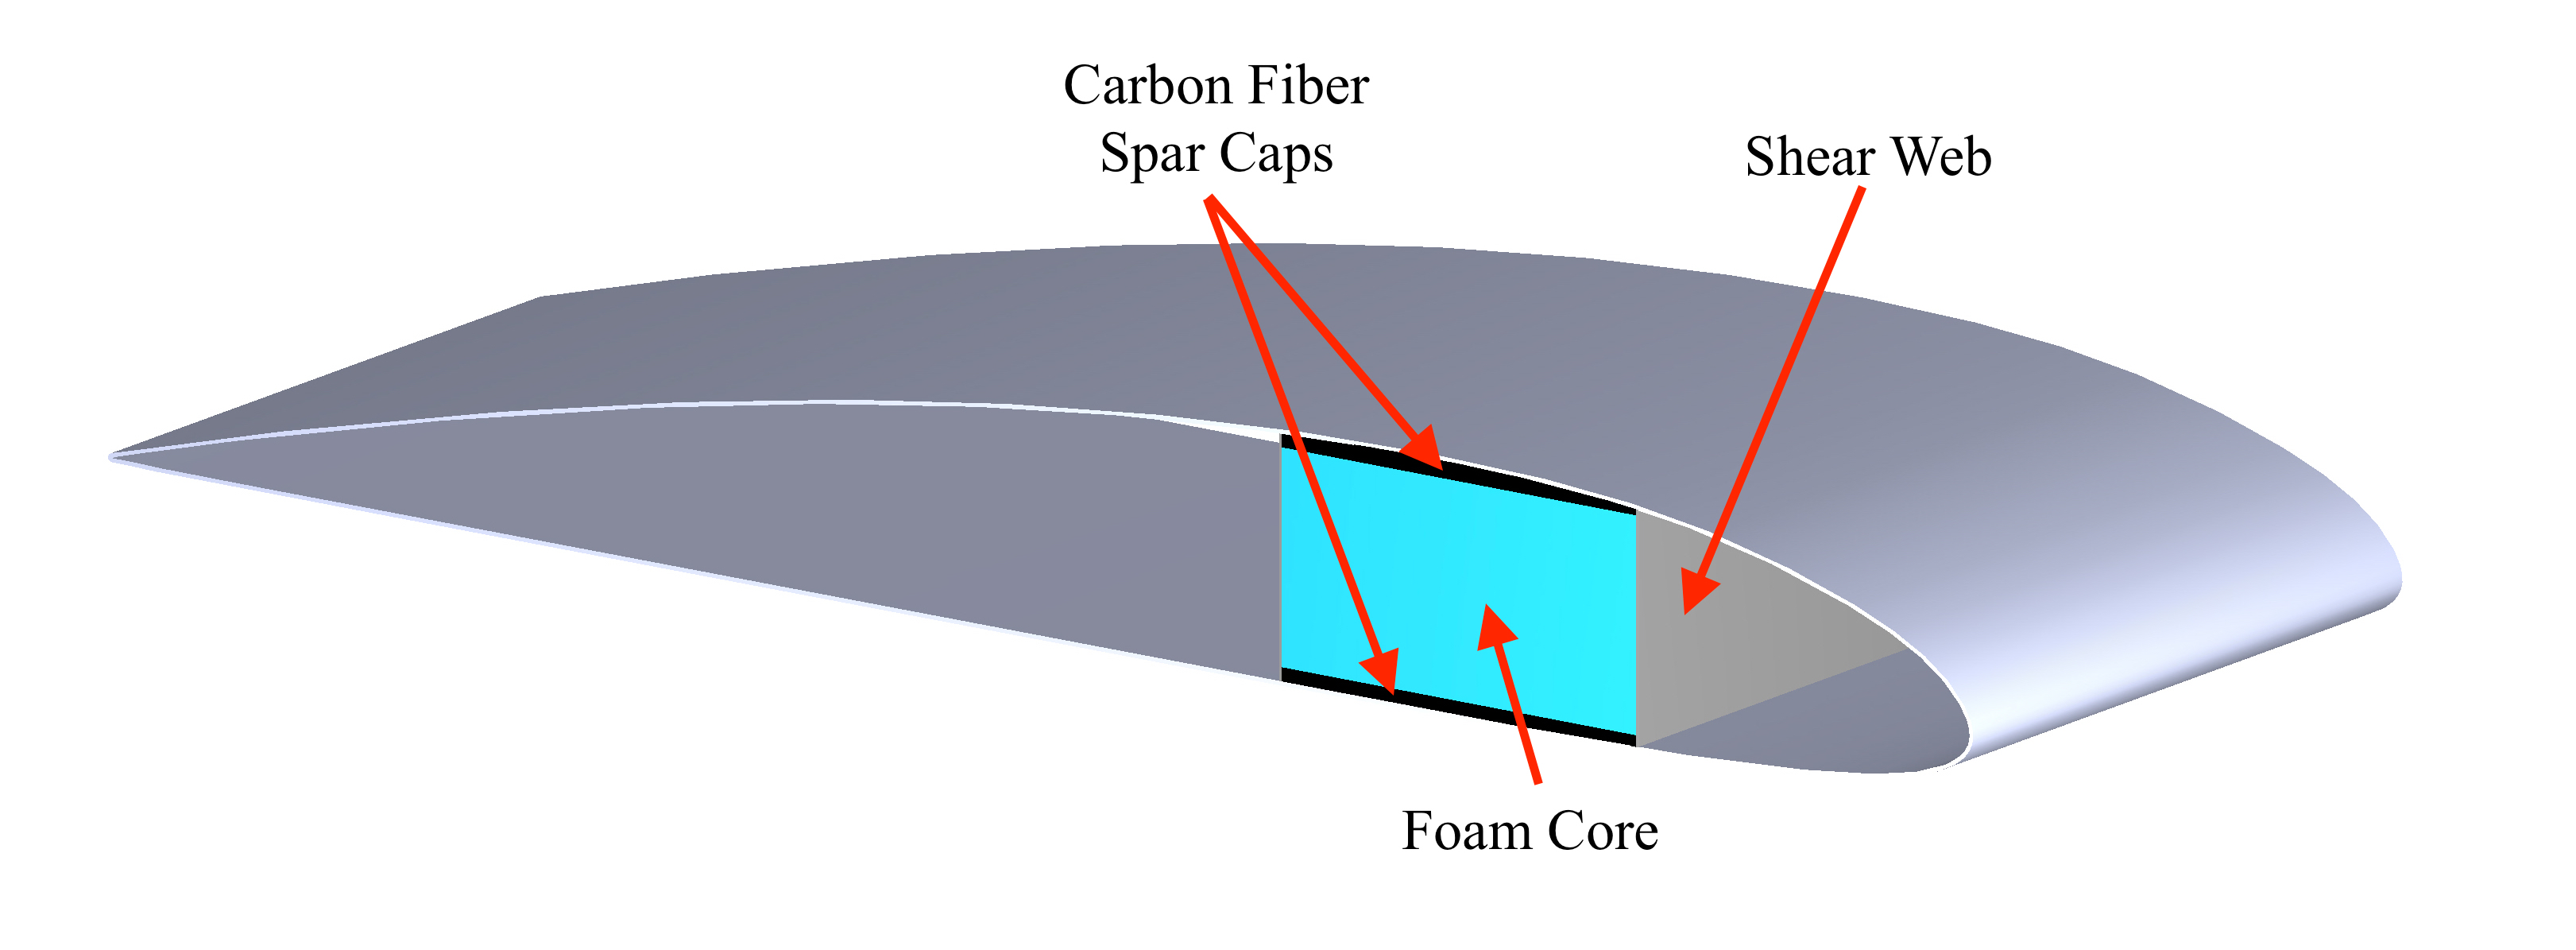
\includegraphics[width=0.8\textwidth]{capspar2.jpg}
    \caption{ \textbf{ Cross sectional view of a cap spar.  The two caps are made of carbon fiber, separated by a foam core. A thin shear web is wrapped around the caps and foam to prevent shearing.}}
	\label{f:capspar}
	\end{center}
\end{figure}

The moment of inertia of the cap spar is modeled by only considering the spar caps, not the foam interior.  
This conservative assumption is made because the contribution of the foam core is much less than that of the spar caps.  
The equation for the moment of inertia\cite{bending} of a cap spar is 

\begin{equation}
    \label{e:moispar}
    I = \frac{w_{\text{cap}}t_{\text{cap}}^3}{6} 2w_{\text{cap}}t_{\text{cap}}\left( \frac{h_{\text{cap}}}{2} + \frac{t_{\text{cap}}}{2} \right)^2
\end{equation}

This equation is not GP compatible.  However, using a first order conservative approximation, the moment of inertia can be simplified to be written in a GP-compatible form, 

\begin{equation}
    \label{e:moispar}
    I \leq 2w_{\text{cap}}t_{\text{cap}}\left(\frac{h_{\text{cap}}}{2}\right)^2
\end{equation}

There are also geometric constraints imposed on the width and thickness.  The total spar cap thickness cannot be greater than the thickness of the airfoil cross section, $\tau_t = 0.115$.  The width of the spar cap is assumed by no greater than 30\% of chord, $\tau_w = 0.3$.

\begin{align}
    \label{e:thickness}
    c(y)\tau_t &\geq h_{\text{cap}} + 2t_{\text{cap}} \\
    \label{e:width}
    c(y)\tau_w &\geq w_{\text{cap}} 
    \end{align}

To match the discretized beam model, the spar cross section can also be written in a discretized form such that each section has a unique width and thickness. 

\begin{align}
    I_i &\leq 2w_{\text{cap}_i}t_{\text{cap}_i}\left(\frac{h_{\text{cap}_i}}{2}\right)^2 \\
    c(y)\tau_t &\geq h_{\text{cap}_i} + 2t_{\text{cap}_i} \\
    c(y)\tau_w &\geq w_{\text{cap}_i} 
\end{align}

The wing spar at the root must be strong enough to withstand the bending root moment and stiff enough to not exceed some deflection limit.  Both constraints are imposed in the optimization model as

\begin{align}
    \label{e:stresscont}
    \sigma_{\text{carbon fiber}} &\geq \mathcal{M}_0 \frac{h_{\text{cap}}+t_{\text{cap}}}{I}\\
    \label{e:defcont}
    w_n &\leq w_{\text{max}}.
\end{align}

The maximum stress for carbon fiber is, $\sigma_{\text{carbon fiber}} = 475$ [MPa].\cite{carbonfiber}
The tip deflection is constrained to be less than 20\% of the half span, $\frac{w_{\text{max}}}{b/2} = 0.2$.

Finally, the weight of the spar cap is computed as

\begin{align}
    \label{e:sparmass}
    \Delta W_i &\geq \rho_{\text{carbon fiber}} w_{\text{cap}_i}t_{\text{cap}_i} \frac{b/2}{n-1}g \\
    \label{e:sparmasssum}
    W_{\text{spar}} &\geq 2 \sum\limits_{1}^{n-1} \Delta W_i
\end{align}

where $\rho_{\text{carbon fiber}} = 1.4$ [g/cm$^3$].\cite{carbonfiber}

\subsection{Wing Skin Weight}

It is assumed that the wing skin is made of carbon fiber.  The weight of the wing skin is 

\begin{equation}
    \label{e:wingskinweight}
    W_{\text{skin}} \geq 2 \rho_{\text{carbon fiber}} S g 
\end{equation}

where $\rho_{\text{carbon fiber}} = 0.043$ [g/cm$^2$].\cite{carbonfiber}

\subsection{Empennage}

An empennage model with a single tail consisting of a tail boom, horizontal and vertical tail, is added to both the solar-electric and gas powered aircraft.  
The empennage adds both weight and drag to the each aircraft.  

The tail boom has a diameter $d$, root wall thickness $t_0$, root moment of inertia $I_0$, modulus $E$, and density $\rho_{\text{carbon fiber}} = 1.4$ [g/cm$^3$], and length $l_{\text{h}}$. 
The total mass and root bending inertia are imposed in the optimization model as 

\begin{align}
    m &\geq \pi \rho_{\text{carbon fiber}} t_0 d l_{\text{h}} \left( 1 + \frac{1}{2} k\right) \\
    I_0 &\leq \pi t_0 d^3/8
\end{align}

where the index $k=0$ corresponds to a uniform wall thickness and stiffness, and $k=1$ corresponds to a linear drop-off to zero.  For both the solar-electric and gas powered aircraft $k=0.8$.  When the tail boom is loaded at the endpoint $x=l_{\text{h}}$, by the horizontal tail lift $L_{\text{h}}$, the end deflection angle follows from standard beam analysis. 

\begin{align}
    \label{e:boomdefl}
    \theta &\geq \frac{L_{\text{h}} l_{\text{h}}^2}{EI_0} \frac{1+k}{2} \\
    L_{\text{h}} &= \frac{1}{2} C_{L_{\text{h}}} \rho V^2 S_{\text{h}}
\end{align}

The horizontal tail is sized to satisfy a horizontal tail volume coefficient condition, $V_{\text{h}} = 0.45$.\cite{aircraftrules}

\begin{equation}
    V_{\text{h}} = \frac{S_{\text{h}}l_{\text{h}}}{Sc}
\end{equation}

% meet a minimum static margin $\text{SM}_{\text{min}} = 0.35$ and minimum desirable c.g. travel range,
% 
% \begin{equation}
%     \label{e:deltacg}
%     \Delta x_{cg} = (x_{cg})_{\text{aft}} - (x_{cg})_{\text{fwd}} = 0.2
% \end{equation}
% 
% A single constraint, whose derivation is explained in Appendix C, minimizes the horizontal tail volume coefficient $V_{\text{w}}$, while meeting the minimum static margin and minimum c.g. travel range,
% 
% \begin{align}
%     \label{e:smcorr}
%     \text{SM}_{\text{min}} + \frac{\Delta x_{cg}}{c} - \frac{C_{M_{	ext{w}}}}{C_{L_{\text{max}}}} &\leq V_{\text{w}} \mathcal{F}_{NE}^{-1} \frac{m_{\text{h}}}{m_{\text{w}}} \left( 1 - \frac{d\epsilon}{d\alpha}\right) + V_{\text{w}} \frac{-(C_{L_{\text{h}}})_{\text{min}}}{C_{L_{\text{max}}}} \\
%     \label{e:htv}
%     V_{\text{w}} &= \frac{S_{\text{h}}}{S} \frac{l_{\text{h}}}{c}
% \end{align}
% 
% Because this equation is not posynomial, it was reformulated as conservative monomial approximation
% 
% \begin{align}
%     1 &\geq z_{\text{SM}_1} \left(\frac{m_{\text{w}} \mathcal{F}_{NE}}{m_{\text{h}} V_{\text{w}}})\right) + \frac{d\epsilon}{d\alpha} \\
%     z_{\text{SM}_2} &\leq V_{\text{w}}\frac{(C_{L_{\text{h}}})_{\text{min}}}{C_{L_{\text{max}}}} \\
%     \label{e:smcorrmon}
%     z_{\text{SM}_1}^{0.48} z_{\text{SM}_1}^{0.52} &\geq \text{SM}_{\text{min}} + \frac{\Delta x_{cg}}{c} - \frac{C_{M_{	ext{w}}}}{C_{L_{\text{max}}}}
% \end{align}
% 
% where the values, 0.48 and 0.52, are chosen as an approximate percentage that each term is of the right hand side of Equation~\eqref{e:smcorrmon}. 

The vertical tail is sized to meet a conservative volume tail coefficient, $V_{\text{v}}= 0.02$,\cite{aircraftrules}

\begin{equation}
    \label{e:vtv}
    V_{\text{v}} = \frac{S_{\text{v}}}{S} \frac{l_{\text{v}}}{b}
\end{equation}

where $l_{\text{v}}$ is the vertical tail moment arm and assume to be equal to the horizontal tail moment arm, $l_{\text{v}} = l_{\text{h}}$.

Both the horizontal and vertical tails are assumed to have a carbon fiber skin and solid foam interior where their respective densities are $\rho_{\text{carbon fiber}} = 0.1$ [g/cm$^2$], $\rho_{\text{foam}} = 1.5$ [lbf/ft$^3$]. 
The weight of the horizontal and vertical tails is

\begin{align}
    \label{e:htweight}
    W_{\text{h}} &= \rho_{\text{foam}} \frac{S_{\text{h}}^2}{b_{\text{h}}} \bar{A} + g\rho_{\text{carbon fiber}} S_{\text{h}} \\
    \label{e:vtweight}
    W_{\text{v}} &= \rho_{\text{foam}} \frac{S_{\text{v}}^2}{b_{\text{v}}} \bar{A} + g\rho_{\text{carbon fiber}} S_{\text{v}}
\end{align}

where $b_{\text{h}}$ and $b_{\text{v}}$ are the spans of the horizontal and vertical tails respectively and $\bar{A}$ is the cross sectional area of the NACA 0008 airfoil.

The drag of the empennage was considered as three separate parts with no interference drag.  The drag of the tail boom was calculated using a turbulent flat plate model,

\begin{align}
    \label{e:boomdrag}
    D_{\text{boom}} &\geq \frac{1}{2} C_f \rho V^2 l_{\text{h}}\pi d \\
    C_f &\geq \frac{0.445}{Re_{\text{boom}}^{0.3}} \\
    Re_{\text{boom}} &= \frac{V\rho l_{\text{h}}}{\mu}
\end{align}

The drag of the horizontal and vertical tails was computed using a GP-compatible fit of XFOIL data for a range of Reynolds numbers and NACA airfoil thicknesses,

\begin{align}
    D_{\text{h}} &\geq \frac{1}{2} c_{d_{\text{h}}} \rho V^2 S_{\text{h}} \\
    D_{\text{v}} &\geq \frac{1}{2} c_{d_{\text{v}}} \rho V^2 S_{\text{v}} \\
    \label{e:taildrag}
    c_{d_{\text{(v,h)}}}^{70.5599} &\geq \num{7.42688d-90} \left( \frac{Re_{\text{(v,h)}}}{\num{1d3}} \right)^{-33.0637}(100 \tau_{\text{(v,h)}})^{18.0419}  \nonumber \\
                 & + \num{5.02826d-163}\left(\frac{Re_{\text{(v,h)}}}{\num{1d3}}\right)^{-18.7959} (100\tau_{\text{(v,h)}})^{53.1879} \\
                 &+ \num{4.22901d-77}\left(\frac{Re_{\text{(v,h)}}}{\num{1d3}}\right)^{-41.1704} (100\tau_{\text{(v,h)}})^{28.4609} \nonumber \\
    Re_{\text{v}} &= \frac{V\rho S_{\text{v}}/b_{\text{v}}}{\mu} \\
    Re_{\text{h}} &= \frac{V\rho S_{\text{h}}/b_{\text{h}}}{\mu} 
\end{align}

where $\tau_{\text{(v,h)}} = 0.08$ is the airfoil thickness. Assuming steady level flight where neither surface is generating lift, the XFOIL data was generated for a zero angle of attack. A comparison of the XFOIL data and Equation~\eqref{e:taildrag} is shown in Figure~\ref{f:taildragpolar}.

\begin{figure}[H]
	\begin{center}
	\includegraphics[width=0.6\textwidth]{taildragpolar.pdf}
    \caption{ \textbf{Comparison of XFOIL data for NACA airfoils to GP-compatible generated fit,~\eqref{e:taildrag}. (Log space RMS error = 0.0173)}}
	\label{f:taildragpolar}
	\end{center}
\end{figure}

\subsection{Elliptcal Fuselage for Gas Powered Aircraft}

For the gas powered aircraft it is assumed that the fuel is carried in an elliptically shaped fuselage.  The fuselage will increase the overall weight and drag of the aircraft.  The solar-electric powered aircraft is assumed to carry the batteries in the wings will therefore have a smal fuselage whose effects will be ignored.  

The driving constraint for the size of the fuselage is to ensure that all of the fuel required for the mission can fit inside the fuselage, 

\begin{equation}
    \label{e:fusevol}
    \mathcal{V}_{\text{fuse}} \geq \frac{W_\text{fuel}}{\rho_\text{fuel}}
\end{equation}

where the fuel is assumed to be Jet A fuel with density $\rho_\text{fuel} = 6.01$ [lbf/gallon].  The volume of the fuselage is constrained by

\begin{equation}
    \label{e:fusevol2}
    \mathcal{V}_{\text{fuse}} \leq \frac{4}{3}\pi \frac{l_{\text{fuse}}}{2}R_{\text{fuse}}^2
\end{equation}

where $l_{\text{fuse}}$ is the length of the fuselage and $R_{\text{fuse}}$ is the radius. Using the length and radius the surface area can be calculated using Thomsen's approxmiation,\cite{ellipsoidSA}

\begin{equation}
    \label{e:fusesa}
    3 \left( \frac{S_{\text{fuse}}}{\pi} \right)^{1.6075} \geq 2(2l_{\text{fuse}}R_{\text{fuse}})^{1.6075} + ((2R_{\text{fuse}})^2)^{1.6075}.
\end{equation}

The weight of the fuselage is based off of the surface area

\begin{equation}
    \label{e:fuseweight}
    W_{\text{fuse}} \geq S_{\text{fuse}} \rho_{\text{carbon fiber}} g
\end{equation} 

where $\rho_{\text{carbon fiber}} = 0.085$ [g/cm$^2$].\cite{carbonfiber}  The surface area is also used to calculate the drag assuming a skin friction based drag model,

\begin{align}
    \label{e:fusedrag}
    D_{\text{fuse}} &\geq C_f k_{\text{fuse}} \frac{1}{2} \rho V^2 S_{\text{fuse}} \\
    C_f &\geq \frac{0.455}{Re^{0.3}}
\end{align}

where $k_{\text{fuse}}$ is the form factor approximated by\cite{raymer}

\begin{equation}
    \label{e:fuseform}
    k_{\text{fuse}} \geq 1 + \frac{60}{(l_{\text{fuse}}/2R_{\text{fuse}})^3} + \frac{(l_{\text{fuse}}/2R_{\text{fuse}})}{400}.
\end{equation}

\subsection{Engine Weight}

The solar-electric powered aircraft has a motor whose weight is based on the approximation\cite{electricengine}

\begin{equation}
    \label{e:electricengine}
    P_{\text{max}} = B_{PM} m_{\text{motor}}
\end{equation}

where $m_{\text{motor}}$ is the motor mass, $P_{\text{max}} \geq P_{\text{oper}}$ is the maximum operating power, and the power to mass ration is $B_{PM} = 4140.8$ [W/kg]. \\

The engine weight of the gas powered aircraft is governed by a simple power law derived from existing two-stroke and four-stroke engines\cite{gasengine}

\begin{equation}
    \label{e:powerlaw}
    \frac{W_{\text{engine}}}{W_{\text{engine-ref}}} = 1.27847 \left(\frac{P_{\text{SL-max}}}{P_{\text{ref}}} \right)^{0.772392}
\end{equation}

where $W_{\text{engine-ref}} = 10$ [lbs] and $P_{\text{ref}} = 10$ [hp].  Equation~\eqref{e:powerlaw} was found using techniques described in Hoburg\cite{fitting}. Equation~\eqref{e:powerlaw} is compared to the data in Figure~\ref{f:powervsweightfit}

\begin{figure}[H]
	\begin{center}
	\includegraphics[width=0.6\textwidth]{powervsweightfit.pdf}
    \caption{ \textbf{ Comparison of power law equation and engine data.  Engine data taken from University of North Dakota technical report.\cite{gasengine} (Log space RMS error = 0.34)}}
	\label{f:powervsweightfit}
	\end{center}
\end{figure}

\subsection{Gas Powered Engine Performance}

Two characteristics of gas engines affect the performance of long-endurance aircraft.  
The first is break specific fuel consumption, $BSFC$; a lower $BSFC$ will result in increased endurance.  
The second is the lapse rate.  
Assuming a propeller driven aircraft and a naturally aispirated engine, as the aircraft reaches higher altitudes, the engine will have decreased available power. 
To account for these two affects a two-stroke, double cylinder engine, the DF70 from RCV Engines Ltd, England, was selected as a representative engine.  
RCV Engines Ltd manufacturing data that was used to generate representative performance curves.\cite{rcvengines}
It is assumed that engines of a similar class will perform similarly to the DF70 engine.  
Thus, this engine performance model is only valid for IC engines.

\subsubsection{Break Specific Fuel Consumption Constraint}

A GP-compatible curve was generated from the DF70 data to relate $BSFC$ and shaft power, 

\begin{equation}
    \label{e:rpmtobsfc}
    \left( \frac{BSFC}{BSFC_{\text{min}}} \right)^{18.5563} \geq \num{8.66321d-3}\left( \frac{P_{\text{shaft}}}{P_{\text{max}}}\right)^{-7.70161} + 1.38628\left( \frac{P_{\text{shaft}}}{P_{\text{max}}} \right)^{1.12921} \\
\end{equation}

where $BSFC_{\text{min}} = 0.3162$ [lb/hp/hr].\cite{rcvengines}
Using this approximations the required shaft power determines the $BSFC$.
A comparison of the GP-compatible approximations to the manufacturing data from RCV engines is presented in Figure~\ref{f:powervsweightfit}. A comparison of the DF70 data provided by RCV Engine Ltd in Figure~\ref{f:powervsweightfit} to the $BSFC$ to power curves in Goering\cite{bsfcperf} verify that this performance curve is representative of engines of a similar class. 

\begin{figure}[H]
	\begin{center}
	\includegraphics[width=0.6\textwidth]{powertobsfcfit.pdf}
 \caption{\textbf{Comparison of GP-compatible approximation to RCV manufacturing data for the DF70 engine.  Function is representative of engine performance for engines of similar size.  The log-space RMS error is 0.007. }}
	\label{f:powervsweightfit}
	\end{center}
\end{figure}

\subsubsection{Engine Lapse Rate Calculation}

The lapse rate $L_{\text{eng}} \leq 1$, is assumed to affect the maximum power output,

\begin{equation}
    \label{e:lapse}
    L_{\text{eng}} = \frac{P_{\text{max}}}{P_{\text{SL-max}}}.
\end{equation}

The lapse is calculated from the required flight altitude $h=15,000$ [ft], prior to the optimization solve using an approximate engine loss rate for normally aspirated engines of 3.5\% hp per 1000 ft,\cite{enginelapse}

\begin{equation}
    \label{e:lapsefit}
    L_{\text{eng}} = 1 - \frac{0.035}{1000 \text{ [ft]}} h.
\end{equation}

\subsection{Climb Constraints}

Because the gas engine is naturally aspirated, as the aircraft climbs there will be less available power.  
The climb constraint ultimately sizes the engine because at the top of climb, when the least amount of power is available, the engine must be big enough to provide the necessary power to meet the minimum climb rate, 

\begin{equation}
    \label{e:climbrate}
    \dot{h} \geq 100 \text{ [ft/min]}.
\end{equation}

The climb rate affects the required thrust, and therefore the required power during climb, 

\begin{equation}
    \label{e:climb}
    T \geq \frac{1}{2} C_D \rho V^2 S + W \frac{\dot{h}}{V}
\end{equation}

where $W$, is the weight of the aircraft during climb.  

\section{Results}

With more detailed structural and performance models the accuracy of the optimization results improves. 
Figure~\ref{f:latvsmtowtrade} was recalculated with the additional constraints included from Section V and is presented in Figure~\ref{f:latvsmtowtradet}. 
The higher fidelity models reveal a more realistic limit to the size of the solar-electirc powered aircraft and actually improve the performance of the gas powered aircraft.

\begin{figure}[H]
 \begin{subfigmatrix}{2}% number of columns
     \subfigure[Gas Powered\label{f:mtowvslatgas}]{\includegraphics{mtowvslatgas.pdf}}
     \subfigure[Solar-Electric Powered\label{f:mtowvslatsolar}]{\includegraphics{mtowvslatsolar.pdf}}
 \end{subfigmatrix}
 \caption{\textbf{ Recalulation of trade study of max take off weight and latitude with more detailed structural and performance models.   }}
 \label{f:latvsmtowtradet}
\end{figure}

One way in which adding higher fidelity models increases the accuracy of the optimization is that higher fidelity models allow new varibles to be solved by the optimizer instead of being inputs. 
For example, the aspect ratio and non-wing drag coefficient, which were previously inputs, can now be optimized with more detailed models.  
At 31 degrees latitude and 90th percentile winds the optimum aspect ratio is $A=32.6$ and the the non-wing drag coefficient is $C_{d_0} = 0.0043$ for the solar-electric powered aircraft.

Additional models also improve the optimization accuracy because of new variable dependencies. 
By adding in a wing structural model, air density has a larger effect on the operating altitude of the solar-electric powered aircraft.  
It might be assumed that because the wind speeds are lowest at 67,000 ft at 31 degrees latitude, that the aircraft will always fly at 67,000 ft.  
Figure~\ref{f:altopersimple} confirms that without a structural model the aircraft will want to fly almost exactly at 67,000 ft.  
However, by adding a structural model larger wings now have a weight penalty and according to Equation~\eqref{e:slfweight}, for the same $C_L$, with a smaller wing, higher air density will generate more lift. 
Therefore, by adding a structural model the optimization seeks a smaller wing to save weight and operates at a lower altitude to increase density. 
Figure~\ref{f:altoper} shows that with a wing structural model the optimum operating point is not at the minimum wind speed. 

\begin{figure}[H]
 \begin{subfigmatrix}{2}% number of columns
     \subfigure[Structural weight fraction\label{f:altopersimple}]{\includegraphics{windaltopersimple.pdf}}
     \subfigure[Detailed structural model\label{f:wstruct}]{\includegraphics{windaltoper.pdf}}
 \end{subfigmatrix}
 \caption{\textbf{Comparison of optimum operating altitude for the solar-electric powered aircraft with and without a detailed structural model.  With only a structural fraction as the structural model the optimum point is at the minimum wind speed.  With a more detailed structural model the optimum operating altitude is not at the minimum wind speed because of variable interaction between wing weight, air density, and wind speed. }}
 \label{f:altoper}
\end{figure}

Higher fidelity results can also been seen using detailed structural and performance models in the gas powered aircraft. 
Interesting, a direct comparison between the simple and detailed optimization models shows a cross over around an endurance of 6.5 days, Figure~\ref{f:simpdetcomp}. The comparison was run at a latitude of 38 degrees and 90th percentile winds.

\begin{figure}[H]
 \begin{subfigmatrix}{2}% number of columns
     \subfigure[Max take off weight comparison\label{f:simpdetcomp}]{\includegraphics{simpdetcomp.pdf}}
     \subfigure[Non-wing drag coefficient comparison\label{f:nonwingdrag}]{\includegraphics{nonwingdrag.pdf}}
 \end{subfigmatrix}
 \caption{\textbf{Comparison of gas powered optimization with and without detailed structural and performance model.  Non-wing drag variation due to Reynolds number effects cause of cross over in Figure~\ref{f:simpdetcomp}. }}
 \label{f:gasdetcomp}
\end{figure}

An analysis of the non-wing drag coefficienct, Figure~\ref{f:nonwingdrag}, reveals that cross over between the static non-wing drag coefficient $C_{d_0}=0.01$, and the more detailed component drag breakdown is one cause of the discrepancy between the detailed and non-detailed optimization models. 
The decrease in non-wing drag, even as the size of the aircraft increases, is due to a Reynolds number effect.  
For a constant airspeed, air density and viscosity, as the aircraft increases in size, Reynolds number will increase which will decrease the non-wing drag coefficient.

\subsection{Solar-electric Powered Trade Space Exploration}

One way analyze the trade space of the solar-electirc powered aircraft it is to change the objective function.  
High efficiency solar cells are expensive and from a manufacturing perspective, a larger aircraft that requires fewer solar cells could be advantageous.
Altering the objective function to solar cell area can show difference configurations that meet the same requirements. 

\begin{figure}[H]
	\begin{center}
	\includegraphics[width=0.6\textwidth]{solarobjcomp.pdf}
    \caption{\textbf{Solar aircraft sizing study for two different objective functions: wing span $b$, and solar cell area $S_{\text{solar}}$. }}
	\label{f:solarobjcomp}
	\end{center}
\end{figure}

For a broader picture of the design space the solar optimization is solved multiple times, producing a set of contour plots for various battery energy densities, solar cell efficiencies, altitudes, and availabilities.  (Figure~\ref{f:solarcontours}) 
The matrix contour plot map is a useful reference tool designed to give understanding to key trade offs in the solar-electric powered aircraft sizing problem.

 \begin{figure}[H]
 \begin{subfigmatrix}{3}% number of columns
  \subfigure[35th Latitude, 80\% Wind Speed]{\includegraphics{bcontourl35a80.pdf}}
  \subfigure[35th Latitude, 85\% Wind Speed]{\includegraphics{bcontourl35a85.pdf}}
  \subfigure[35th Latitude, 90\% Wind Speed]{\includegraphics{bcontourl35a90.pdf}}
  \subfigure[30th Latitude, 80\% Wind Speed]{\includegraphics{bcontourl30a80.pdf}}
  \subfigure[30th Latitude, 85\% Wind Speed]{\includegraphics{bcontourl30a85.pdf}}
  \subfigure[30th Latitude, 90\% Wind Speed]{\includegraphics{bcontourl30a90.pdf}}
  \subfigure[25th Latitude, 80\% Wind Speed]{\includegraphics{bcontourl25a80.pdf}}
  \subfigure[25th Latitude, 85\% Wind Speed]{\includegraphics{bcontourl25a85.pdf}}
  \subfigure[25h Latitude, 90\% Wind Speed]{\includegraphics{bcontourl25a90.pdf}}
 \end{subfigmatrix}
 \caption{ \textbf{Matrix of contour plots of battery energy density and solar cell efficiency vs wing span for solar-electric powered aircraft. Each point on the graph corresponds to a unique design.} }
 \label{f:solarcontours}
\end{figure}


\section{Conclusion}

Using geometric programming as a form of evaluation of the design space, high level intuition and understanding about design trade studies for long-endurance aircraft and their driving requirements is achieved.  
One high level discovery is the important of wind speed.  
If station keeping at all times during the flight is critical to the mission of a proposed aircraft, then that requirement is more likely to be met by a gas-powered architecture.
However, if that constraint can be relaxed such that the aircraft only needs to station keep for 80\% of then time, then for certain latitudes, a solar powered aircraft could achieve greater endurance.
An unsurprising discovery is the sensitivity of the solar-powered aircraft to the battery energy density and solar cell efficiency.  Using higher energy density batteries can result in significant weight and performance savings.  
The rapid solve time of geometric programming is able to present these trade studies and give intuition into design trades by quantifying the disparity in performance between two options.
While the results of these findings are dependent on the accuracy of the models used in the optimization, it is shown that higher fidelity models can be incorporated to increase accuracy.


% produces the bibliography section when processed by BibTeX
\bibliography{biblibrary}
\bibliographystyle{aiaa}

\section*{Appendix A}

\subsection{Wind Speed Constraints}

The each wind speed constraint follows the following form

\begin{equation}
    \label{e:windspeedgen}
    \left(\frac{V_{\text{wind}}}{V_{\text{ref}}}\right)^{\alpha} \geq c_1 \rho^{e_{1,1}}p_{\text{wind}}^{e_{1,2}} + c_2 \rho^{e_{2,1}}p_{\text{wind}}^{e_{2,2}} + c_3 \rho^{e_{3,1}}p_{\text{wind}}^{e_{3,2}} + c_4 \rho^{e_{4,1}}p_{\text{wind}}^{e_{4,2}}
\end{equation}

Table~\ref{t:windvals} lists the values of the coefficients and exponents of Equation~\eqref{e:windspeedgen} for latitudes 20-60. 

\tiny
\begin{longtable}{lccccccccccccc} \\
\label{t:windvals} \\
    \toprule
    \toprule
    \caption{Wind Speed Function Coefficients and Exponents} \\
    Latitude & $c_1$ & $e_{1,1}$ & $e_{1,2}$ & $c_2$ & $e_{2,1}$ & $e_{2,2}$ & $c_3$ & $e_{3,1}$ & $e_{3,2}$ & $c_4$ & $e_{4,1}$ & $e_{4,2}$ & $\alpha$ \\
    \midrule
20 & 9.77e-15 & -8.45 & 53.1 & 5.26e+04 & 9.98 & 6.26 & 1.97e+03 & 7.66 & 39.3 & 3.9e-14 & -7.26 & 10.6 & 5.53\\
21 & 1.01e-13 & -7.88 & 47.9 & 6.66e-13 & -6.62 & 9.18 & 8.09e+04 & 9.61 & 5.48 & 1.36e+03 & 7.04 & 35.8 & 5.03\\
22 & 1.12e+05 & 9.65 & 5.29 & 1.53e-13 & -7.75 & 47.6 & 7.58e-13 & -6.64 & 8.9 & 2.03e+03 & 7.11 & 35 & 5.06\\
23 & 2.68e+03 & 7.11 & 34 & 1.07e-12 & -6.61 & 8.67 & 1.35e+05 & 9.6 & 5.09 & 4.2e-13 & -7.46 & 48.6 & 5.08\\
24 & 4.81e+03 & 7.4 & 33.6 & 6.8e-13 & -7.25 & 48.3 & 1.95e+05 & 9.81 & 5.08 & 4.84e-13 & -6.87 & 8.91 & 5.31\\
25 & 2.14e-12 & -6.86 & 48 & 6.28e+03 & 7.5 & 33.3 & 2.02e+05 & 9.8 & 5.12 & 3.1e-13 & -7.06 & 9.17 & 5.48\\
26 & 7.48e+03 & 7.51 & 34.7 & 2.95e+05 & 9.9 & 5.26 & 3.13e-13 & -7.14 & 9.52 & 7.03e-12 & -6.51 & 51.4 & 5.59\\
27 & 3.62e+05 & 10 & 5.44 & 7.09e-12 & -6.54 & 51.1 & 1.29e-13 & -7.44 & 9.71 & 8.93e+03 & 7.57 & 36.3 & 5.82\\
28 & 7.9e-14 & -7.65 & 9.68 & 8.89e+03 & 7.5 & 36.9 & 3.28e+05 & 9.95 & 5.58 & 6.85e-12 & -6.64 & 49.3 & 5.96\\
29 & 6.97e-14 & -7.79 & 9.85 & 2.3e+05 & 9.71 & 5.72 & 7.67e+03 & 7.34 & 36.4 & 1.15e-11 & -6.58 & 50.3 & 6.02\\
30 & 4.2e-14 & -8.05 & 10.2 & 1.29e+05 & 9.38 & 6 & 5.8e+03 & 7.15 & 36.4 & 1.44e-11 & -6.62 & 52.2 & 6.12\\
31 & 2.17e-12 & -7.2 & 57.6 & 9.1e+03 & 7.56 & 40.5 & 1.22e-15 & -9.09 & 11.8 & 1.26e+05 & 9.68 & 7.21 & 6.89\\
32 & 6.21e+04 & 9.3 & 7.9 & 3.54e-12 & -7.12 & 58.1 & 5.23e-16 & -9.45 & 12.2 & 6e+03 & 7.32 & 42.5 & 7.07\\
33 & 1.86e-16 & -9.86 & 12.8 & 2.81e+04 & 8.91 & 8.68 & 3.98e+03 & 7.13 & 44.5 & 8.01e-12 & -6.89 & 58.7 & 7.28\\
34 & 9.95e+03 & 8.43 & 9.54 & 4.7e-17 & -10.4 & 13.5 & 2.66e+03 & 6.97 & 46.7 & 1.19e-11 & -6.79 & 61 & 7.55\\
35 & 2.92e+03 & 7.59 & 9.37 & 1.58e-10 & -6.07 & 60.4 & 4.05e-16 & -9.88 & 13.2 & 1.05e+03 & 6.33 & 46.2 & 7.21\\
36 & 456 & 5.77 & 45 & 3.4e-15 & -9.35 & 12.8 & 834 & 6.79 & 8.98 & 1.23e-09 & -5.52 & 58.8 & 6.92\\
37 & 5.15e-14 & -8.63 & 12.1 & 225 & 5.94 & 8.34 & 8.45e-09 & -5.03 & 57.5 & 196 & 5.19 & 43.2 & 6.52\\
38 & 84.8 & 4.63 & 41.6 & 4.69e-08 & -4.61 & 55.3 & 67.8 & 5.13 & 7.68 & 8.55e-13 & -7.87 & 11.2 & 6.1\\
39 & 1.65e-11 & -7.05 & 10.1 & 35.7 & 4.06 & 40.1 & 22.4 & 4.33 & 6.95 & 2.55e-07 & -4.18 & 51.7 & 5.6\\
40 & 16.7 & 3.57 & 38.4 & 2.62e-10 & -6.28 & 9.05 & 1.32e-06 & -3.75 & 48 & 8.73 & 3.63 & 6.25 & 5.11\\
41 & 3.42e-09 & -5.56 & 7.84 & 3.93 & 2.99 & 5.53 & 8.86e-06 & -3.19 & 43.4 & 11.2 & 3.27 & 37.3 & 4.6\\
42 & 2.06 & 2.42 & 4.8 & 4.04e-08 & -4.87 & 6.63 & 10.3 & 3.16 & 35.8 & 6.03e-05 & -2.61 & 39.2 & 4.07\\
43 & 13.8 & 3.32 & 34.9 & 0.000428 & -2.01 & 36.7 & 1.27 & 1.93 & 4.09 & 4.21e-07 & -4.22 & 5.58 & 3.55\\
44 & 0.929 & 1.54 & 3.39 & 19.9 & 3.54 & 34.2 & 3.77e-06 & -3.6 & 4.62 & 0.00191 & -1.54 & 34.3 & 3.03\\
45 & 0.0061 & -1.16 & 32.6 & 2.75e-05 & -3.04 & 3.83 & 0.783 & 1.24 & 2.76 & 27.5 & 3.75 & 34.2 & 2.55\\
46 & 35.2 & 3.97 & 32.9 & 0.000197 & -2.47 & 3.02 & 0.758 & 1.01 & 2.13 & 0.0176 & -0.791 & 30.5 & 2.04\\
47 & 0.00143 & -1.89 & 2.2 & 42.2 & 4.28 & 28.5 & 0.816 & 0.811 & 1.47 & 0.046 & -0.43 & 28.9 & 1.49\\
48 & 0.926 & 0.622 & 0.814 & 0.0108 & -1.29 & 1.34 & 0.106 & -0.0538 & 28.2 & 57.2 & 4.99 & 20 & 0.895\\
49 & 56.5 & 5.67 & 11.3 & 0.128 & 0.183 & 27.4 & 0.95 & 0.455 & 0.349 & 0.0533 & -0.793 & 0.695 & 0.445\\
50 & 0.869 & 0.355 & 0.148 & 24.1 & 5.47 & 7.62 & 0.0838 & 0.217 & 27.1 & 0.139 & -0.487 & 0.358 & 0.229\\
51 & 4.88 & 4.99 & 5.72 & 0.657 & 0.238 & 0.0196 & 0.0293 & 0.214 & 27.7 & 0.345 & -0.21 & 0.116 & 0.0703\\
52 & 0.00842 & 0.166 & 28 & 0.834 & 4.31 & 4.86 & 0.615 & -0.0754 & 0.0355 & 0.383 & 0.186 & -0.0168 & 0.0212\\
53 & 0.307 & 0.168 & -0.0266 & 0.335 & 3.6 & 4.1 & 0.687 & -0.0538 & 0.0264 & 0.00564 & 0.12 & 27.7 & 0.0155\\
54 & 0.00497 & 0.0916 & 27.5 & 0.223 & 3.09 & 3.42 & 0.54 & -0.067 & 0.0346 & 0.449 & 0.0992 & -0.0245 & 0.0144\\
55 & 0.429 & -0.0809 & 0.0543 & 0.00527 & 0.0771 & 27.7 & 0.206 & 2.77 & 3.25 & 0.553 & 0.0722 & -0.0305 & 0.0158\\
56 & 0.134 & 2.62 & 3.28 & 0.628 & 0.0434 & -0.0319 & 0.00348 & 0.0804 & 28 & 0.358 & -0.072 & 0.0644 & 0.0106\\
57 & 0.00421 & 0.0943 & 28 & 0.0734 & -0.168 & 0.207 & 0.905 & 0.0123 & -0.013 & 0.155 & 2.47 & 3.06 & 0.0128\\
58 & 0.00709 & 0.107 & 28.8 & 0.0366 & -0.258 & 0.474 & 0.253 & 2.33 & 2.98 & 0.921 & 0.00373 & -0.013 & 0.0225\\
59 & 0.0242 & 0.892 & 28.4 & 0.000155 & -1.21 & 16.1 & 0.945 & -0.0147 & 0.0161 & 0.188 & 1.98 & 1.32 & 0.0233\\
60 & 0.0173 & 0.691 & 28.1 & 0.948 & -0.0136 & 0.015 & 0.209 & 2.15 & 1.6 & 7.54e-05 & -1.41 & 14.3 & 0.0222 \\
\bottomrule
\end{longtable}
\normalsize

\section*{Appendix B}

\subsection{Discussion on the use of the \emph{JH01} airfoil}

The \emph{sd7032} airfoil was redesigned to prevent drag creep by weakening the pressure spike associated with premature separation at higher Reynolds numbers.  
Figure~\ref{f:jhcps} shows the pressure distributions generated in XFOIL of the \emph{JH01} airfoil at $C_L=0.0$ and $C_L=1.35$ with $Re=3e5$.
The redesigned airfoil was named \emph{JH01}. We would like to thank Mark Drela who helped in the redesign.

\begin{figure}[H]
 \begin{subfigmatrix}{2}% number of columns
     \subfigure[$C_L=0.0$\label{f:cpmin}]{\includegraphics{cpmin.pdf}}
     \subfigure[$C_L=1.35$\label{f:cpmax}]{\includegraphics{cpmax.pdf}}
 \end{subfigmatrix}
 \caption{\textbf{ Pressure coefficient plots at the minimum and maximum expected $C_L$ at Reynolds number, $Re=3e5$.  }}
 \label{f:jhcps}
\end{figure}

% \section*{Appendix C}
% 
% To derivation of Equation~\eqref{e:smcorr} begins with the moment about the aircraft's center of mass
% 
% \begin{align}
%     \label{e:mcenter}
%     M_{cg} &= M_{\text{w}} + (x_{cg} - x_{ac})L_{\text{w}} - l_{\text{h}} L_{\text{h}} \\
%     \label{e:eq6}
%     \frac{M_{cg}}{qSc} = C_m &= C_{m_{\text{w}}} + \frac{x_{cg} - x_{ac}}{c} C_{L_W} - V_{\text{w}} C_{L_{\text{h}}}
% \end{align}
% 
% It is assumed that the tail boom's effective root location is at the wing's aerodynamic center $x_{ac}$, and that the tail's pitching moment about its own aerodynamic center is negligible. 
% 
% Using moment and lift approximations
% 
% \begin{align}
%     C_{m_{\text{w}}} &= constant \\
%     C_{L_W} &= C_{L_{W_0}} + m_{\text{w}} \alpha \\
%     \label{e:eq10}
%     C_{L_{\text{h}}} &= C_{L_{h_0}} + m_{\text{h}} \left[\left( 1 - \frac{d\epsilon}{d\alpha}\right) - \theta \right] + C_{L_{h_{\delta}}}\delta_e \\
%     m_{\text{w}} &= \frac{2\pi}{1 + 2/AR_{\text{w}}} \\
%     m_{\text{h}} &= \frac{2\pi}{1 + 2/AR_{\text{h}}}
% \end{align}
% 
% where $\epsilon$ is the wing's downwash angle seen at the tail. Using a vortex approximation and neglecting taper effects, we can estimate
% 
% \begin{equation}
%     \frac{d\epsilon}{d\alpha} = \frac{m_{\text{w}}}{4\pi} \frac{c}{l_{\text{h}}}
% \end{equation}
% 
% so that \eqref{e:eq10} can be written as
% 
% \begin{equation}
%     C_{L_{\text{h}}} = m_{\text{h}} \left[\left( 1 - \frac{d\epsilon}{d\alpha}\right) - \frac{qS_{\text{h}}l_{\text{h}}^2}{EI_0}(1-\frac{1}{2}k) C_{L_{\text{h}}}\right] + C_{L_{h_{\delta}}}(\delta_e - \delta_{e_0}) 
% \end{equation}
% 
% This can be further simplified by defining a tail boom flexibility factor $\mathcal{F}$.
% 
% \begin{align}
%     C_{L_{\text{h}}} &= \mathcal{F}^{-1} m_{\text{h}} \left( 1 - \frac{d\epsilon}{d\alpha}\right) \alpha + \mathcal{F}^{-1} C_{L_{h_{\delta}}}(\delta_e - \delta_{e_0}) \\
%     \mathcal{F} &= 1 + m_{\text{h}} \frac{qS_{\text{h}}l_{\text{h}}^2}{EI_0}(1-\frac{1}{2}k) 
% \end{align}
% 
% Using the wing lift coefficient and the recast tail lift coefficient, the pitching moment is equation and derivative are given as follows.
% 
% \begin{align}
%     C_m &= C_{m_{\text{w}}} + \frac{x_{cg} - x_{ac}}{c} (C_{L_{W_0}} + m_{\text{w}} \alpha) - V_{\text{w}} \left[ \mathcal{F}^{-1} m_{\text{h}} \left( 1 - \frac{d\epsilon}{d\alpha}\right) \alpha + \mathcal{F}^{-1} C_{L_{h_{\delta}}}(\delta_e - \delta_{e_0})\right] \\
%     \frac{dC_m}{d\alpha} & = \frac{x_{cg} - x_{ac}}{c} m_{\text{w}}  - V_{\text{w}} \mathcal{F}^{-1} m_{\text{h}} \left( 1 - \frac{d\epsilon}{d\alpha}\right) 
% \end{align}
% 
% Now by dividing by $dC_{L_W}/d\alpha = m_{\text{h}}$, which defines the static margin
% 
% \begin{equation}
%     -\frac{dC_m/d\alpha}{dC_{L_W}/d\alpha} = \text{SM} = V_{\text{w}} \mathcal{F}^{-1} \frac{m_{\text{h}}}{m_{\text{w}}} \left( 1 - \frac{d\epsilon}{d\alpha}\right) - \frac{x_{cg} - x_{ac}}{c}
% \end{equation}
% 
% The case for meeting the minimum static margin requirement is at the never-exceed dynamic pressure $q_{NE}$ and when the c.g is at its aft-most position.
% 
% \begin{equation}
%     \text{SM}_{\text{min}} = V_{\text{w}} \mathcal{F}_{NE}^{-1} \frac{m_{\text{h}}}{m_{\text{w}}} \left( 1 - \frac{d\epsilon}{d\alpha}\right) - \frac{(x_{cg})_{\text{aft}} - x_{ac}}{c} 
% \end{equation}
% 
% Dividing Equation~\eqref{e:eq6} by $C_{L_W}$, gives a requirement on the tail lift coefficient required to achieve a pitch trim condition $C_m=1$
% 
% \begin{equation}
%     0 = \frac{C_{m_{\text{w}}}}{C_{L_W}} + \frac{x_{cg} - x_{ac}}{c} - V_{\text{w}} \frac{C_{L_{\text{h}}}}{C_{L_W}}
% \end{equation}
% 
% The pitch authority requirement is that at the forward-most c.g. position and maximum lift with the tail lift coefficient equal to the most-negative allowable value $(C_{L_{\text{h}}})_{\text{min}}$. Combining the static margin and pitch authority requirement results in the horizontal tail sizing equation 
% 
% \begin{align}
%     \text{SM}_{\text{min}} + \frac{\Delta x_{cg}}{c} - \frac{C_{M_{\text{w}}}}{C_{L_{\text{max}}}} &\leq V_{\text{w}} \mathcal{F}_{NE}^{-1} \frac{m_{\text{h}}}{m_{\text{w}}} \left( 1 - \frac{d\epsilon}{d\alpha}\right) + V_{\text{w}} \frac{-(C_{L_{\text{h}}})_{\text{min}}}{C_{L_{\text{max}}}} \\
% \end{align}
% 
% where $\Delta x_{cg} = (x_{cg})_{\text{aft}} - (x_{cg})_{\text{fwd}}$.

\end{document}

% - Release $Name:  $ -
